
%\documentclass{svjour3}                     % onecolumn (standard format)
%\documentclass[smallcondensed]{svjour3}     % onecolumn (ditto)
\documentclass[smallextended]{svjour3}       % onecolumn (second format)
%\documentclass[twocolumn]{svjour3}          % twocolumn
%
\smartqed  % flush right qed marks, e.g. at end of proof
%
\usepackage{graphicx}
%
\usepackage{amsmath,amssymb}
\usepackage{times}
\usepackage{enumerate}

\usepackage{mathrsfs}
% \usepackage{mathptmx}      % use Times fonts if available on your TeX system
%
% insert here the call for the packages your document requires
%\usepackage{latexsym}
% etc.
%
% please place your own definitions here and don't use \def but
% \newcommand{}{}
%

% \newtheorem{thm}{Theorem}[section]
% \newtheorem{cor}[thm]{Corollary}
% \newtheorem{lem}[thm]{Lemma}
% \newtheorem{prob}[thm]{Problem}

% %% Numbered objects of "non-theorem" style (text roman):
% \theoremstyle{definition}
% \newtheorem{defn}[thm]{Definition}
% \newtheorem{rem}[thm]{Remark}
% \newtheorem{exa}[thm]{Example}

%% Equations numbered by section:

\numberwithin{equation}{section}

%%%% Put your macros here:

%% Ticketing System
\usepackage{etoolbox}
\usepackage{xparse}
\NewDocumentCommand{\openTickets}{ > {\SplitList {,} } m }{\ProcessList{#1}{\BoolInit}}
\newcommand{\BoolInit}[1]{\providetoggle{#1}\toggletrue{#1}}
\newcommand{\todo}[2]{%
  \providetoggle{#1}%
    \iftoggle{#1}{%
    {\color{red}#2}%
    }{#2}%
}

\usepackage{tikz}
\usetikzlibrary{arrows,positioning,patterns,decorations.pathreplacing}

%% Ticket list
\openTickets{Manuel:convHull,Manuel:wlog,Manuel:invertability:assumption,Mark:log:bounds,Mark:proof:cor15,Manuel:proof:rewritten,Manuel:generic}

\providecommand{\norm}[1]{\left\|#1\right\|}
\providecommand{\abs}[1]{\left|#1\right|}
\providecommand{\span}{\text{span}}
\providecommand{\conv}{\text{conv}}
\providecommand{\epi}{\text{epi}}
\providecommand{\rk}[1]{\text{rank}\left(#1\right)}

\newcommand*{\Resize}[1]{\resizebox{\columnwidth}{!}{$#1$}}

\DeclareFontFamily{U}{mathx}{\hyphenchar\font45}
\DeclareFontShape{U}{mathx}{m}{n}{
      <5> <6> <7> <8> <9> <10> gen * mathx
      <10.95> mathx10 <12> <14.4> <17.28> <20.74> <24.88> mathx12
      }{}
\DeclareSymbolFont{mathx}{U}{mathx}{m}{n}
\DeclareFontSubstitution{U}{mathx}{m}{n}
\DeclareMathSymbol{\temp}{\mathbin}{mathx}{'341}
\newcommand{\bigominus}{\raisebox{10pt}{$\temp$}}

% \newcommand{\todo}[1]{\textcolor{blue}{#1}}
\newcommand{\highlight}[1]{\textcolor{red}{#1}}

% Insert the name of "your journal" with
% \journalname{myjournal}
%
\begin{document}

\title{Explicit Operations on Parametrised Polytopes}%\thanks{Grants or other notes
%about the article that should go on the front page should be
%placed here. General acknowledgments should be placed at the end of the article.}
%\subtitle{Do you have a subtitle?\\ If so, write it here}

%\titlerunning{Short form of title}        % if too long for running head

\author{Rainer M. Schaich
\and 
Mark Cannon}

%\authorrunning{Short form of author list} % if too long for running head

\institute{R. M. Schaich: Department of Engineering Science,
  University of Oxford, Oxford, OX1 3PJ, UK; \email{rainer.schaich@eng.ox.ac.uk}
\and
M. Cannon:  Department of Engineering Science,
  University of Oxford, Oxford, OX1 3PJ, UK; \email{mark.cannon@eng.ox.ac.uk}}

\date{\today}

\maketitle


\begin{abstract}
The Pontryagin set difference is an operation between two sets that is used to calculate sets of safe operation in diverse applications including game theory and robust control.
%
We consider a particular class of set-valued maps; for this we introduce the property of parametric convexity and present some of its analytic framework.
%
In order to guarantee the convexity of the difference of a convex set and a set-valued map it proves necessary and sufficient that the set-valued map is parametrically convex.
%
For generic piecewise polyhedral set-valued maps we show that parametric convexity is equivalent to a constant combinatorial structure of all its realisations.
%
We present a computational method for verifying parametric convexity of a piecewise polyhedral set-valued map as well as a way to calculate the parametric Pontryagin difference between a polyhedron and a piecewise polyhedral set-valued map.
%
Two examples are given to illustrate the presented methodology.

\keywords{Parametric convexity \and Piecewise affine set-valued map \and Pontryagin difference \and Parametrised polytopes}

\subclass{52B55 \and 52A41 \and 90C25}
% 52A20 Convex sets in $n$ dimensions (including convex hypersurfaces)
% 52B55 Computational aspects related to convexity
% 52B11 $n$-dimensional polytopes
% 52A41 Convex functions and convex programs
% 52A30 Variants of convex sets (star-shaped, ($m, n$)-convex, etc.)
% 90C25 Convex programming
% 68U05 Computer graphics; computational geometry
% 52C45 Combinatorial complexity of geometric structures
\end{abstract}

% \linenumbers

\section{Introduction}
%
The Pontryagin difference was originally introduced (under the 
name Minkowski difference) as a set theoretic tool
in~\cite{Hadwiger:1950,Hadwiger:1957}. 
%However in the years since the term Minkowski difference has often been used to refer to a different operation.
%
It was implicitly reintroduced in the context of
differential games in~\cite{Pontryagin:1966}, where it was used to characterise safe sets for which strategies could be found which keep elements inside some second set for all possible adversary actions.
%
Since its introduction, the usage of the Pontryagin difference has been extended beyond applications in differential games to various scenarios in which safe sets are needed that withstand some perturbation.
%
See for example~\cite{blanchini:2007} for a its use as a robust
control analysis tool in several different contexts and under the name
(set-)erosion. It has also found use in morphological image analysis, e.g.~\cite{Haralick:1987}.
%

When the Pontryagin difference has to be performed explicitly by numerical algorithms, it is usually assumed that the respective sets are polytopic, since it is not possible to operate on general sets explicitly.
%
Algorithms to determine the Pontryagin difference between two
polytopes do not require more complex computation than the solving of
linear programs~\cite{Kolmanovsky:1998,Kerrigan:2003}, and their
analytical properties are well-known, see e.g.~\cite{blanchini:2007,Haralick:1987,Kolmanovsky:1998}.
%
The sets on which these operations can be performed are fixed
predetermined polytopes but, due to their physical interpretation in
terms of safe sets, it can be desirable to extend the class of sets on which these operations can be performed.
%
For this purpose we consider the case in which the subtrahend is a
set-valued map with a polytopic realisation.

General set-valued maps have been studied analytically and various results are available in the literature, see e.g.~\cite{Aubin:2009}.
%
However, computational aspects of operations on general set-valued
maps are largely unknown. We refer to~\cite{Finzel:2000} for some results for polyhedral set-valued maps.
%
In this paper we present a particular class of set-valued map for which the Pontryagin difference can be computed explicitly.
%
The set-valued maps we consider are parametrised polytopes with a property we introduce as \emph{parametric convexity} which allows us to guarantee that the \emph{parametric Pontryagin difference} is convex for all convex minuend sets.
%
We provide the computational framework to allow us to perform parametric Pontryagin differences explicitly.

The paper is structured as follows:
%
In Section~\ref{sec:preliminaries} we summarise preliminaries that are
required throughout the paper. In
Section~\ref{sec:parametric:convexity} we introduce parametric
convexity, which is the essential ingredient for all subsequent
analysis, and provide analytic results for set operations. 
We refine and extend these results for the case of set-valued maps with polyhedral realisations in Section~\ref{sec:polyhedral:maps}.
%
Section~\ref{sec:computational:methods} elaborates on how to determine whether a polyhedral map is in fact parametrically convex and how to perform operations on such set-valued maps, these concepts are then illustrated in Section~\ref{sec:numerical:examples} by two examples and finally we conclude the paper in Section~\ref{sec:conclusion}.


Throughout this paper we refer to the the real $d$-dimensional parameter space as $Y\subseteq\mathbb R^d$, the $n$-dimensional realisation space as~$Z\subseteq\mathbb R^n$ and its power set~$\mathscr P(Z)$.
%
We denote the integer range~$\{1,\dots,m\}$ by~$\mathbb N_m$ and index sets by $\mathcal A,\,\mathcal J$ or $\mathcal I$, the complement of a subset of an index set $\mathcal I\subset\mathcal A$ is denoted by $\bar{\mathcal I}=\mathcal A\setminus\mathcal I$, the objects $a_{\mathcal I}$ and $b_{\mathcal I}$ denote the matrix and the column vector with rows given by the row vectors $a_i$ and the scalar values $b_i$ with $i\in\mathcal I$.
%
By $f\vert_\Omega$ we mean $f$ evaluated only $\Omega$, a ball centred around $c$ of radius $r$ is denoted by $B_r(z)=\{x:\norm{x-z}_2\leq\epsilon\}$ with the Euclidean norm $\norm{\cdot}_2$.
%
The Minkowski sum~\cite{Minkowski:1911} of the sets $X_1,X_2$ is denoted by $X_1\oplus X_2$, for a $d_2$ dimensional set $X$ the projection onto $\mathbb R^{d_1}$ with $d_1\leq d_2$ is denoted by $\pi_{d_1}(X) = \{x\in\mathbb R^{d_1}:\exists \tilde x\in\mathbb R^{d_2-d_1} (x,\tilde x)\in X\}$.
%
For a polytopic set $X$ the set of its vertices is denoted by $\text{vert}(X)$.
%
\section{Preliminaries}\label{sec:preliminaries}

Throughout the paper we deal with set-valued maps, i.e. functions that map an element of a metric space~$Y$ to a subset of a metric space~$Z$, that is $f:Y\mapsto\mathscr P(Z), Y\ni y\rightarrow f(y)\subset Z$. 
%
A detailed presentation on properties of set-valued maps is beyond the scope of this paper and we refer to~\cite{Aubin:2009}, here we only assume that the set-valued map is continuous in the sense that its \emph{graph}
%
\begin{equation}
  \mathscr G(f) = \{(y,z)\in Y\times Z: z\in f(y)\}
\end{equation}
%
has a continuous boundary, i.e. for every bounded point $(y,z)\in\partial\mathscr G(f)$ the boundary $\partial\mathscr G(f)$ is locally given by the graph of a continuous function.
%
We only consider set-valued maps with convex images, i.e. maps for which $z_1,z_2\in f(y)\Rightarrow \lambda z_1+(1-\lambda)z_2\in f(y)$ for all $\lambda\in[0,1]$ holds for all $y\in Y$.

An important subset of such set-valued maps are such that their realisations are polytopic, i.e. $f(y)$ is a polytope for all $y\in Y$, in particular we study maps which depend on the \emph{parameter} in a piecewise affine way.
%
The graph of such maps is given by a union of polytopes, they have been studied in~\cite{Finzel:2000}.
%
We will make statements about \emph{generic} such maps, that is properties which are structurally stable in the sense that if~$f(y)$ has a particular property than there exists an open neighbourhood $U\ni y$ such that $f(\tilde y)$ has the same property for all $\tilde y\in U$, furthermore the set of points for which the property does not hold is of measure zero.
%
In the course of this paper it will be self evident what the set of points is, where the property of interest fails, in particular a lower dimensional polyhedron and we therefore omit a measure theoretic treatment of our assumption.

The particular property we require is \emph{simplicity}, for each $y\in Y$ the set $f(y)$ is a polytope and each of its vertices~$v(y)$ is supported by a minimal number of hyperplanes, i.e. there exists a linear system defining the set~$f(y) = \{z:A(y)z\leq b(y)\}$ and each vertex $v(y)$ is defined by $n$ hyperplanes $A_{\mathcal I}(y)v(y)=b_{\mathcal I}(y)$ and $A_{\bar{\mathcal I}}(y)v(y)<b_{\bar{\mathcal I}}(y)$.
%
It is easy to see, that if $A(\cdot)$ and $b(\cdot)$ are continuous in $y$, then $\mathcal I$ locally defines a vertex, i.e. the combinatorial structure of a simple polytope is structurally stable and therefore being simple is a generic property of a polytope.


The induced graph~$G(P)$ of a polytope~$P$ is the graph with vertices and edges that coincide with the vertices and edges of the polytope itself~\cite{Bondy:2008}.
%
In this paper we only use one property of induced graphs, namely the \emph{Perles Conjecture}~\cite{Kalai:1988}:
\emph{For a simple polytope~$P$ the graph~$G(P)$ determines the combinatorial structure of~$P$.}

\section{Parametric Convexity}\label{sec:parametric:convexity}

In this section we define the property of \emph{parametric convexity} in the context of set-valued maps. 
%
This property is then used to demonstrate the convexity of a generalised Pontryagin difference operation (see e.g.~\cite{Hadwiger:1950,blanchini:2007}). 
%
% In this section we refer to sets $Y\subseteq\mathbb R^d$ and $Z\subseteq\mathbb R^n$.
%
\begin{definition}[Parametric Convexity]\label{def:parametric:convexity}
Let $\mathcal W:Y\rightarrow \mathscr P(Z)$, where $Y\ni p\mapsto \mathcal W(p) \subset Z$, be a continuous set-valued map. The map $\mathcal W$ is called \emph{parametrically convex} if it satisfies
%
  \begin{equation}\label{eq:def:parametrically:convex}
  \mathcal W(\lambda p_1 + (1-\lambda)p_2)\subseteq\lambda \mathcal W(p_1) \oplus (1-\lambda) \mathcal W(p_2).
\end{equation}
for all $p_1,p_2\in Y$ and $\lambda\in (0,1)$.
\end{definition}
%
Notice that Definition~\ref{def:parametric:convexity} does not require convexity of~$\mathcal W(p)$. 
%
However, recall that we will only consider maps~$\mathcal W$ for which $\mathcal W(p)$ is convex for all fixed $p\in Y$.
%
A similar definition was given in~\cite{Hadwiger:1957} for scalar families of sets ($d=1$), however the results presented are not directly related.

\subsection{Properties of Parametrically Convex Maps}\label{ssec:properties:of:p:convex:maps}
%
We begin by introducing an equivalent characterisation of parametric convexity that provides an insight into the geometrical properties of 
set-valued maps satisfying~\eqref{eq:def:parametrically:convex}.
%
This is based on a description of parametric convexity in terms of conditions on the graph~$\mathscr G(\mathcal W)$ of a set-valued map.
%
\begin{definition}\label{def:graph:of:map}
Let $\mathcal W:Y\rightarrow \mathscr P(Z)$ be a continuous set-valued map
such that $\mathcal W(p)$ is convex for all $p\in Y$, then 
%
\begin{equation*}\begin{aligned}
\text{int}(\mathscr G(\mathcal W)) = \{(p,z) \in Y\times Z : \forall \zeta\in\mathbb R^n\;\exists \epsilon>0, \, z+\epsilon \zeta\in \mathcal W(p) \}
\end{aligned}\end{equation*}
%
denotes the \emph{interior} of its graph and
%
\[
  \partial \mathscr G(\mathcal W) = \mathscr G(\mathcal W)\setminus \textup{int}(\mathscr G(\mathcal W))
\]
%
its \emph{boundary};
%
furthermore for any $(p,z)\in\partial\mathscr G(\mathcal W)$ the \emph{normal cone} is defined as 
%
\[
  \mathcal N_{\mathcal W} (p,z) = \{\zeta \in\mathbb R^n: \zeta^T (y - z) \leq 0, \;  \forall y\in \mathcal W(p) \} .
\]
%
\end{definition}
%
\begin{remark}
%
Note that the normal cone in Definition~\ref{def:graph:of:map} is defined in the space of the \emph{set variable} $z\in Y$ rather than \emph{graph variable} $(p,z)\in Y\times Z$.
%
Furthermore, the normal cone $\mathcal N_{\mathcal W} (p,z)$ is the set of normals to all hyperplanes that contain $z$ but no other points in $\mathcal W(p)$.
%
\end{remark}
%
The central idea connecting parametric convexity of a set valued map $\mathcal W$ with properties of its graph $\mathscr G(\mathcal W)$ is stated next.
%
\begin{theorem}\label{thm:p:convexity:graph}
  A map $\mathcal W$ such that $\mathcal W(p)\ni 0$ for all $p\in Y$
  is parametrically convex iff for all $(p_1,z_1), (p_2,z_2)\in\partial\mathscr G(\mathcal W)$
  with
  %$p_1\neq p_2$ and
  $\mathcal N_{\mathcal W}(p_1,z_1)\cap\mathcal N_{\mathcal W}(p_2,z_2)\neq\emptyset$,
%
\begin{equation}\label{eq:graph:def:p:convexity}
\lambda (p_1,z_1) + (1-\lambda) (p_2,z_2) \not\in\textup{int} (\mathscr G(\mathcal W))
\end{equation}
%
holds for all $\lambda\in(0,1)$.
%
\end{theorem}
%
\begin{proof}
  %
  Consider the set $S$, defined for given $\lambda\in (0,1)$ and $p_1,p_2\in Y$ by
  \[
    S = \lambda \mathcal{W}(p_1) \oplus (1-\lambda) \mathcal{W}(p_2) 
      = \bigl\{ z : \lambda z_1 + (1 - \lambda) z_2, \ z_1 \in\mathcal W(p_1), \ z_2 \in\mathcal W(p_2) \bigr\} .
  \]
  % \begin{align*}
  %   S &= \lambda \mathcal{W}(p_1) \oplus (1-\lambda) \mathcal{W}(p_2) \\
  %     &= \bigl\{ z : \lambda z_1 + (1 - \lambda) z_2, \ z_1 \in\mathcal W(p_1), \ z_2 \in\mathcal W(p_2) \bigr\} .
  % \end{align*}
  We first show that $z\in \partial S = S \setminus \textup{int}(S)$ if and only if
  % \begin{equation}\label{eq:Scond}
  %   z = \lambda z_1 + (1 - \lambda) z_2
  %   \quad \text{and} \quad
  %   \mathcal N_{\mathcal W}(p_1,z_1) \cap \mathcal N_{\mathcal W}(p_2,z_2) \neq \emptyset 
  % \end{equation}
  $z = \lambda z_1 + (1 - \lambda) z_2$ for some $z_1\in\partial \mathcal W(p_1)$ and $z_2\in\partial \mathcal W(p_2)$ such that $\mathcal N_{\mathcal W}(p_1,z_1) \cap \mathcal N_{\mathcal W}(p_2,z_2) \neq \emptyset$.
  %
  
  Specifically, if $z\in \partial S$ then $z\in S$ and there exists $\zeta\in\mathbb R^n$ such that $z + \epsilon \zeta \notin S$ for all $\epsilon > 0$.
  %
  From this it follows that $z = \lambda z_1 + (1-\lambda ) z_2$ for $z_1\in\partial \mathcal W(p_1)$ and $z_2\in\partial \mathcal W(p_2)$ and there exists $n\in \mathbb R^n$ such that for all $\mu \in [0,1]$ we have
  \begin{equation}\label{eq:normal_cone_cond}
    n^T \bigl( \mu \zeta_1 + (1-\mu) \zeta_2 \bigr) \leq 0 
  \end{equation}
  for all $\zeta_1$and $\zeta_2$ such that $n_1^T\zeta_1 \leq 0$ and $n_2^T\zeta_2 \leq 0$ for all $n_1\in\mathcal N_{\mathcal W}(p_1)$ and $n_2\in\mathcal N_{\mathcal W}(p_2)$. Note that these conditions are equivalent to the requirement that the normal cone to $S$ at $z$ is non-empty.
  %
  Clearly $n\in \mathcal N_{\mathcal W}(p_1)$ (since $\mu = 1$ in (\ref{eq:normal_cone_cond}) gives $n^T\zeta_1 \leq 0$) and similarly $n\in \mathcal N_{\mathcal W}(p_2)$ (since $\mu = 0$ in (\ref{eq:normal_cone_cond}) gives $n^T\zeta_2 \leq 0$), and hence $\mathcal N_{\mathcal W}(p_1,z_1) \cap \mathcal N_{\mathcal W}(p_2,z_2) \neq \emptyset$ is necessary for $z\in\partial S$.
  %
  Furthermore $n\in \mathcal N_{\mathcal W}(p_1)\cap \mathcal N_{\mathcal W}(p_2)$ is also sufficient for (\ref{eq:normal_cone_cond}) and hence also $z\in\partial S$.
  %

  If $\lambda z_1 + (1-\lambda ) z_2 \in\partial S$, then (\ref{eq:graph:def:p:convexity}) is equivalent to $\mathcal W\bigl(\lambda p_1 + (1-\lambda) p_2 \bigr) \subseteq S$, and so proof is completed by applying the preceding argument for all $(p_1,z_1) \in\partial\mathscr G(\mathcal W)$ and $(p_2,z_2)\in\partial\mathscr G(\mathcal W)$, and all $\lambda\in (0,1)$.
  \qed
% %
% Assume~\eqref{eq:graph:def:p:convexity} holds for $(p_1,z_1),(p_2,z_2)\in\partial\mathscr G(\mathcal W)$.
% %
% Then the extension of the definition of the Minkowski functional (see e.g.~\cite{Rudin:91}) to the graph $\mathscr G(\mathcal W)$,
% \[
% \mu_{\mathscr G(\mathcal W)} \bigl(
% \mathcal W(p), z \bigr)
% := \min_\mu \{\mu \geq 0 : z \in \mu \mathcal W(p)\},
% \]
% yields $\mu_{\mathscr G(\mathcal W)}\left(\mathcal W(\lambda p_1 + (1-\lambda)p_2),\lambda z_1+(1-\lambda)z_2\right)\geq1$ for all $\lambda\in(0,1)$. Therefore $\lambda z_1 + (1-\lambda) z_2$
% lies either outside the set $\mathcal W(\lambda p_1+(1-\lambda)p_2)$ or on its boundary for all $\lambda\in(0,1)$, and hence the set of all possible interpolation points 
% %
% \[
% \begin{split}
%   \lambda \mathcal W(p_1)\oplus (1-\lambda)\mathcal W(p_2) = \{z : z=\lambda z_1 + (1-\lambda) z_2, z_1\in\mathcal  W(p_1),\, z_2\in\mathcal W(p_2)\}
% \end{split}
% \]
% %
% contains the set $\mathcal W(\lambda p_1 + (1-\lambda)p_2)$ for all $\lambda\in(0,1)$.
% %
% Furthermore, since $\lambda(p_1,z_1)+(1-\lambda)(p_2,z_2)\not\in \text{int}(\mathscr G(\mathcal W))$ and both $(p_1,z_1)$ and $(p_2,z_2)$ lie on the boundary, either $z_1-z_2$ or $z_2-z_1$ is outward facing for both $\mathcal W(p_1)$ and $\mathcal W(p_2)$; therefore either $z_1-z_2$ or $z_2-z_1$ lies in both $\mathcal N_{\mathcal W}(p_1,z_1)$ and $\mathcal N_{\mathcal W}(p_2,z_2)$ and hence also in their intersection.

% Now suppose that $\mathcal W$ is parametrically convex and that~\eqref{eq:graph:def:p:convexity} is not satisfied for 
% some $(p_1,z_1),(p_2,z_2)\in\partial\mathscr G(\mathcal W)$ with $\mathcal N_{\mathcal W}(p_1,z_1)\cap\mathcal N_{\mathcal W}(p_2,z_2)\neq\emptyset$, 
% %
% i.e.~that there exists $\epsilon>0$ such that the ball
% $B_\epsilon(\lambda z_1 + (1-\lambda)z_2 )$
% is contained in $\mathcal W(\lambda p_1 + (1-\lambda)p_2)$ for some $\lambda \in (0,1)$.
% %
% But this implies that $\lambda z_1 + (1-\lambda) z_2 + \epsilon\zeta \in \mathcal W(\lambda p_1+(1-\lambda)p_2)$  for all $\zeta\in\mathbb R^n$ such that $\|\zeta\| = 1$, whereas
% $\mathcal N_{\mathcal W}(p_1,z_1)\cap\mathcal N_{\mathcal W}(p_2,z_2)\neq\emptyset$ implies that there exists 
% $\zeta \in\mathcal N_{\mathcal W}(p_1,z_1)\cap\mathcal N_{\mathcal W}(p_2,z_2)$ which cannot be represented as
% $\zeta =\lambda \zeta_1+
% (1-\lambda)\zeta_2$
% with $z_1 + \epsilon \zeta_1\in\mathcal W(p_1)$ and $z_2  + \epsilon \zeta_2\in\mathcal W(p_2)$.
% %
% It follows that $\mathcal W$ cannot be parametrically convex.
% \qed
\end{proof}
%

Condition~\eqref{eq:graph:def:p:convexity} requires that the graph $\mathscr G(\mathcal W)$ is non-convex.
%
Indeed it is shown next that if $\mathscr G(\mathcal W)$ is strictly convex at any $(p,z)\in\partial \mathscr G (\mathcal W)$, then~\eqref{eq:graph:def:p:convexity} is violated and 
$\mathcal W$ cannot be parametrically convex.

%
\begin{corollary}\label{thm:inequalities:convex:concave}
%
Let $\mathcal W(p):=\{z\in\mathbb R^n: r(p,z)\leq0\}$ define a set-valued
map where 
$r: \mathbb R^d \times\mathbb R^n \rightarrow \mathbb R$, $(p,z)\mapsto r(p,z)$ is a continuous function which is convex in $z \in\mathbb R^n$, 
then $\mathcal W$ is parametrically
convex iff the function $r$ is concave in $p\in\mathbb R^d$.
%
\end{corollary}
%
\begin{proof}
First note that $r(p,z)$ is assumed to be a convex function of $z$ for any given value of $p$ so that $\mathcal W(p)$ is a convex set for each $p\in\mathbb R^d$.
%
Suppose that, for given $z\in\mathbb R^n$, $r(p,z)$ is a non-concave (i.e. 
strictly convex) function of $p$, for all $p$ in some region $\Omega\subseteq\mathbb R^d$. 
%
Then any convex subset $\mathcal C\subseteq\Omega$ will be such that $\mathscr 
G(\mathcal W)\vert_{\mathcal C}$ is a convex set.
%
Furthermore, for any $(p_1,z_1),(p_2,z_2)\in \partial\mathscr G(\mathcal W)\vert_{\mathcal C}$ we have
$\lambda (p_1,z_1) + (1-\lambda) (p_2,z_2) \in\mathrm{int} (\mathscr G(\mathcal W))\vert_{\mathcal C}$ for all $\lambda\in(0,1)$ since
$\mathscr G(\mathcal W)\vert_{\mathcal C}$ is strictly convex in $p$.
%
Hence~\eqref{eq:graph:def:p:convexity} is violated in this case, implying that $r(p,z)$ cannot be a non-concave function of $p$ in any non-empty set $\Omega$ if $\mathcal W$ is parametrically convex. 
%
Conversely, if $r(p,z)$ is concave in $p$ for all $p\in\mathbb R^d$, then the conditions of Theorem~\ref{thm:p:convexity:graph} necessarily hold.
\qed
\end{proof}
%
It is useful to be able to perform set certain set operations on set-valued maps, therefore we define the parametric Pontryagin difference:
%
\begin{definition}[Parametric Pontryagin Difference]\label{def:parametric:pontryagin:difference}
  Let $S\subseteq Z$ and let $\mathcal W:Z\to\mathscr P(Z)$ be a continuous set-valued map such that
  $\mathcal W(p)$ is convex for all $p\in Z$, then the \emph{parametric Pontryagin difference} 
  $S\ominus \mathcal W(S)$ is defined
%
\begin{equation}\label{eq:definition:parametric:pontryagin:difference}
    S\ominus \mathcal W(S) = \bigl\{z\in Z: \{z\} \oplus \mathcal W(z)\subseteq S\bigr\}.
  \end{equation}
%
\end{definition}
%
By a slight abuse of notation, $\mathcal{W}(S)$ is used in~(\ref{eq:definition:parametric:pontryagin:difference}) to indicate that $\mathcal{W}$ is a set-valued map and that $S\ominus\mathcal{W}(S)$ denotes the parametric Pontryagin difference, rather than a fixed set and the conventional Pontryagin difference. 
%
In fact the definition~(\ref{eq:definition:parametric:pontryagin:difference}) indicates that $S\ominus \mathcal{W}(S)$ only depends on the value of $\mathcal{W}(z)$ on a subset of $S$. 
%
%
For the parametric Pontryagin difference of a convex set and a parametrically convex map we 
have the following result.
%
\begin{theorem}\label{thm:convexity:of:pontryagin:difference}
Let $\mathcal W: Z\rightarrow\mathscr P(Z)$ be a given set-valued map, then the parametric Pontryagin difference $S \ominus \mathcal W(S)$ is convex for every convex $S\subseteq Z$ if and only if $\mathcal W$ is parametrically convex.
\end{theorem}
% \begin{theorem}\label{thm:convexity:of:pontryagin:difference}
%   Let $S\subseteq X$ be a convex set and let $\mathcal W:X\rightarrow\mathscr P(X)$ be a parametrically convex point-to-set
%   map such that $\mathcal W(p)$ is convex for all $p\in X$, then $S\ominus \mathcal W(S)$ is convex.
% \end{theorem}
%
\begin{proof}
To prove convexity of $S^\prime =  S\ominus \mathcal W( S)$ when $\mathcal W$ is parametrically convex we pick any $z_1,z_2\in S^\prime$, then
the definition of the parametric Pontryagin difference gives
\begin{equation}
  \{z_i\} \oplus \mathcal W(z_i) \subseteq S,\; i=1,2 
\end{equation}
%
and it can be verified that $S^\prime$ is convex by showing that line segments between all possible $z_1$ and $z_2$ are subsets of $S^\prime$. In particular, for all $\lambda \in (0,1)$ we have
\begin{align*}
  \{ \lambda z_1 + &(1-\lambda)z_2
  \}\oplus \mathcal W\left( \lambda z_1 + (1-\lambda)z_2\right)\\
  \subseteq&\left\{ \lambda z_1 + (1-\lambda)z_2
  \right\}\oplus \lambda \mathcal W(z_1) \oplus (1-\lambda)
  \mathcal W(z_2)\\
 = &\lambda\underbrace{(\{z_1\}\oplus \mathcal W(z_1))}_{\subseteq S}\oplus
  (1-\lambda)\underbrace{(\{z_2\}\oplus \mathcal W(z_2))}_{\subseteq S}\\
  \subseteq& S
\end{align*}
%
(where the last inclusion results from the convexity of $S$), and it follows that
$\lambda z_1 + (1-\lambda) z_2 \in S^\prime$ for all $\lambda \in (0,1)$. 
%the property, which follows from Definition~\ref{def:parametric:pontryagin:difference}, that $S\subseteq Z$.
%

To demonstrate that parametric convexity of $\mathcal W$ is necessary for convexity of $S\ominus \mathcal W(S)$, suppose that condition~(\ref{eq:def:parametrically:convex}) does not hold and choose $z_1,z_2$ so that $\mathcal W(\lambda z_1 + (1-\lambda) z_2) \not\subseteq \lambda \mathcal W(z_1) \oplus (1-\lambda) \mathcal W (z_2)$ for some $\lambda \in (0,1)$. Then there exists a value of $\lambda\in(0,1)$ such that
\begin{align*}
  \{ \lambda z_1 + (1-&\lambda)z_2
  \}\oplus \mathcal W\left( \lambda z_1 + (1-\lambda)z_2\right)\\
  % \not\subseteq&\left\{ \lambda z_1 + (1-\lambda)z_2
  % \right\}\oplus \lambda \mathcal W(z_1) \oplus (1-\lambda)
  % \mathcal W(z_2)\\
 \not\subseteq &\lambda\bigl(\{z_1\}\oplus \mathcal W(z_1)\bigr)\oplus
  (1-\lambda)\bigl(\{z_2\}\oplus \mathcal W(z_2)\bigr) .
\end{align*}
Therefore if $S$ is a convex polyhedron constructed so that $\{z_1\}\oplus\mathcal W(z_1)$ and $\{z_2\}\oplus\mathcal W(z_2)$ contain points lying on the same facet of $S$ (this is always possible if $S^\prime=S\ominus \mathcal W(S)$ has a non-empty interior), then there exists $\lambda \in (0,1)$ such that $\lambda z_1 + (1-\lambda) z_2 \notin S^\prime$.
\qed
\end{proof}
%
Theorem~\ref{thm:convexity:of:pontryagin:difference} provides necessary and sufficient conditions for convexity of the parametric Pontryagin difference. 
%
Later we will show that the parametric Pontryagin difference between a polyhedral set and a piecewise polytopic set-valued map is itself polyhedral.
%
%
%
%
\section{Polyhedral maps}\label{sec:polyhedral:maps}
%
%
%
%
In this section we discuss set-valued maps~$\mathcal W$ for which every realisation~$\mathcal W(p)$ is polyhedral and in particular we study~$\mathcal W$ which depend on $p\in Y$ in a piecewise affine way. 
%
To the authors' best knowledge the literature on piecewise polyhedral sets is limited to~\cite{Finzel:2000}, however properties of general set-valued maps are known and applicable, see e.g.~\cite{Aubin:2009}.
%
\begin{remark}
%
Notice that the boundary of a polytope is almost everywhere locally convex (i.e. concave but not strictly concave) and locally strictly convex around lower dimensional faces (vertices, edges, etc.).
%
This trivial but important fact is exploited throughout the following statements. 
%
As long as the boundary $\partial\mathscr G(\mathcal W)$ is locally affine in $p\in Y$, Corollary~\ref{thm:inequalities:convex:concave} applies. 
%
Conversely if the boundary $\partial\mathscr G(\mathcal W)$ is locally given by more than one affine function in $p\in Y$ (determined by linear inequalities), then it is locally strictly convex and can therefore not be parametrically convex.
\end{remark}
%
\begin{corollary}\label{thm:polytopic:set:not:p:convex}
The polytopic parametric set-valued map $\mathcal W(p):=\{z: a_i z + b_i p\leq c_i \; \forall i\in\mathbb N_m\}$
is not parametrically convex for any non-zero matrix $B^T = [\begin{matrix} b_1^T & \cdots & b_m^T\end{matrix}]$.
\end{corollary}
%
\begin{proof}
If $B\neq 0$, then the graph
%
\begin{equation*}
	\mathscr G(\mathcal W) = \{(p,z):a_i z + b_i p\leq c_i \; \forall i\in\mathbb N_m\} ,
\end{equation*}
%
is convex and violates the conditions of Theorem~\ref{thm:p:convexity:graph}.
\qed
\end{proof}
%
We now present the central theorem of this work, which holds for piecewise affine polytopic set-valued maps which are generic, which implies two things, their realisation is simple and further no more than one structural component changes at a time. 
%
The second assumption will become clearer in the proof of the central statement for piecewise affine polytopic set-valued maps and makes the statement of Theorem~\ref{thm:p:convexity:graph} more specific.
%
\begin{corollary}\label{thm:p:convexity:PWA:set:constant:num:verts}
The generic piecewise affine polytopic parametric set-valued valued map 
%
\begin{equation}\label{eq:definition:PWA:polytopic:set:general}
  \mathcal W(p) := \Bigl\{z\in\mathbb R^n: a_i z \leq \max_{k}\{b_{i,k} + c_{i,k}p\} \; \forall i\in\mathbb N_m \Bigr\}
\end{equation}
%
is parametrically convex iff the number of vertices, $v_\kappa(p)$, and rays, $r_\eta(p)$, of~$\mathcal W(p)$ is constant for almost all $p\in Y$.
\end{corollary}
%
\begin{proof}
For clarity this proof is divided into three parts:
\begin{enumerate}
\item Note that $h_i(p) = \max_{k} \{b_{i,k} + c_{i,k}p\}$ is a multi-parametric linear program (mpLP),
the solution of which is a piecewise affine function $h_i(p) = b_{i,k^\ast_i} + c_{i,k^\ast_i}p$, where $k^\ast_i(p)$ is piecewise constant on a polyhedral complex, see e.g.~\cite{spjotvold:2005}.
%
This means that there exists a finite partition of $Y\subseteq\mathbb R^d$ into convex polyhedra 
$\mathcal P_j$ such that $\bigcup_{j\in\mathcal I} \mathcal P_j = Y$ and 
${\bf{k}}^\ast(p) = (k_1^\ast(p),\dots,k_m^\ast(p))$ is constant for all $p \in \mathcal P_j$.
%
Hence the graph $\mathscr G(\mathcal W)$ is given by a finite union of polyhedra
%
\begin{equation*}
  \mathscr G(\mathcal W) = \bigcup_{j\in\mathcal I} \left\{z: a_i z \leq b_{i,k_i^\ast} + c_{i,k_i^\ast}p \; \forall i \in\mathbb N_m \right\}\bigr\vert_{\mathcal P_{j}}
\end{equation*}
%
and it follows that if the number of vertices or rays changes within any partition $\mathcal P_j$ then $\mathscr
G(\mathcal W)\vert_{\mathcal P_j}$ is a strictly convex polyhedron and Corollary~\ref{thm:polytopic:set:not:p:convex} applies.
%
\item Our attention is therefore concentrated on the boundaries of partitions $\mathcal P_j$, at points $p\in\mathcal P_{j_1} \cap \mathcal P_{j_2}$ where 
%some mpLP changes its solution, i.e. 
$\bigl(b_{i,k_i^\ast} + c_{i,k_{j_1}^\ast} p\bigr)\bigr\rvert_{\mathcal P_{j_1}} = 
\bigl(b_{i,k_{j_2}^\ast} + c_{i,k_{j_2}^\ast} p\bigr)\bigr\rvert_{\mathcal P_{j_2}}$.
%
Notice that a vertex $v_\kappa(p)$ is defined by \emph{active} and \emph{inactive} inequalities, namely $\mathcal A_\kappa(p)$ and
$\bar{\mathcal A}_\kappa(p)$ respectively, where
%
\begin{equation*}\begin{split}
  a_i v_\kappa(p) &= b_{i,k_i^\ast} + c_{i,k_i^\ast} p \quad\forall i\in\mathcal A_\kappa(p)\\
  a_i v_\kappa(p) &< b_{i,k_i^\ast} + c_{i,k_i^\ast} p \quad\forall i\in\bar{\mathcal A}_\kappa(p) .
\end{split}\end{equation*}
%
Since $\mathcal W(p)$ is simple almost everywhere in~$Y$, i.e. each vertex is defined by exactly $n$ active inequalities, we have $\abs{\mathcal A_\kappa(p)}=n$ for all $p\in Y$ and all $\kappa$.
%
Furthermore, since~$\mathcal W(p)$ is generic, only one element of ${\bf{k}}^\ast\vert_{\mathcal P_{j_1}}$
and ${\bf{k}}^\ast\vert_{\mathcal P_{j_2}}$ for neighbouring $\mathcal P_{j_1}$ and $\mathcal P_{j_2}$ differs, that is, there exists a single index $i\in\mathbb N_m$ such that $k_i^\ast\vert_{\mathcal P_{j_1}}\neq k_i^\ast\vert_{\mathcal P_{j_2}}$.
%
Hence, in order for the number of vertices to change, there must be a hyperplane $fp=g$, such that the number of vertices for $fp \leq g$ is 
$N$ and for $fp>g$ is at least $N+1$.
%
It follows from the previous discussion that $\{p:fp=g\} = \textup{aff}\{\mathcal P_{j_1}\cap\mathcal P_{j_2}\}$ for some $j_1\neq j_2$.
%
In order for vertices $v_{\kappa_1}(p)$ and $v_{\kappa_2}(p)$ to merge, the index sets $\mathcal A_{\kappa_1}(p)$ and $\mathcal A_{\kappa_2}(p)$ have to differ by only one 
element, i.e.~$\mathcal A_{\kappa_1}(p) = \mathcal J\cup \{s\}$ and $\mathcal A_{\kappa_2}(p) = \mathcal J\cup\{u\}$ if $fp>g$.
%
Furthermore, for $p$ such that $fp\leq g$ we have $v_{\kappa_1}(p)=v_{\kappa_2}(p)$, implying that $\mathcal A_{\kappa_1}(p) = 
\mathcal A_{\kappa_2}(p)$.
%
Since only one change in the active index set is considered (due to non-degeneracy assumptions), we must have
$\mathcal A_{\kappa_1}(p) = \mathcal A_{\kappa_2}(p) = \mathcal J \cup \{s,u\}$.
%
Hence on the hyperplane $fp=g$, both the maximising index ${\bf{k}}^\ast(p)$ and the active index sets $\mathcal A_{\kappa_1}(p)$ 
and $\mathcal A_{\kappa_2}(p)$ must change, which implies that this problem is degenerate.
%
\item In order for a degenerate graph $\mathscr G(\mathcal W)$ to be parametrically convex, the vertices $v_{\kappa_1}(p)$ and $v_{\kappa_2}(p)$ must be identical for $fp\leq g$, and in particular their dependence on $p$ has to be identical.
%
This can be expressed using the implicit function theorem as follows
%
\begin{align*}
  \frac{d}{dp}\left(  a_{\mathcal J\cup \{s\}} v_{\kappa_1}(p) - b_{\mathcal J\cup \{s\}} - 
  c_{\mathcal J\cup \{s\},{\bf{k}}^\ast} p\right) &= 0\\
  \frac{d}{dp}\left(  a_{\mathcal J\cup \{u\}} v_{\kappa_2}(p) - b_{\mathcal J\cup \{u\}} - 
  c_{\mathcal J\cup \{u\},{\bf{k}}^\ast} p\right) &= 0
\end{align*}
%
which implies
\begin{align*}
  a_{\mathcal J\cup \{s\}} \frac{dv_{\kappa}}{dp} &= c_{\mathcal J\cup \{s\},{\bf{k}}^\ast}\\
  a_{\mathcal J\cup \{u\}} \frac{dv_{\kappa}}{dp} &= c_{\mathcal J\cup \{u\},{\bf{k}}^\ast}
\end{align*}
%
and since we can assume that the inequalities are non-redundant for some right hand side, we find that 
%
\begin{equation}\label{eq:derivative:condition:on:index:sets}
  \frac{dv_\kappa}{dp} = a_{\mathcal J\cup \{s\}}^{-1}c_{\mathcal J\cup \{s\},{\bf{k}}^\ast} = 
  a_{\mathcal J\cup \{u\}}^{-1}c_{\mathcal J\cup \{u\},{\bf{k}}^\ast}
\end{equation}
%
has to hold for the degenerate graph to remain parametrically convex.
%
To complete the proof we note that~\eqref{eq:derivative:condition:on:index:sets} is a degenerate condition, in the sense that an arbitrarily small perturbation will result in $v_{\kappa_1}(p) \neq v_{\kappa_2}(p)$, and we therefore disregard this possibility.
\qed
\end{enumerate}
\end{proof}
%
It is worth pointing out that Corollary~\ref{thm:p:convexity:PWA:set:constant:num:verts} can be reformulated in a numerically useful way:
%
\begin{corollary}\label{thm:combinatorical:equivalence:alternative}
The generic set~$\mathcal W(p)$ defined by~\eqref{eq:definition:PWA:polytopic:set:general} is parametrically convex if and only if it is combinatorially equivalent for any $p_1,p_2\in Y\subseteq\mathbb R^d$ almost everywhere, i.e.\ $\mathcal W(p_1)\cong\mathcal W(p_2)$.
\end{corollary}
%
\begin{proof}
Two polyhedra are combinatorially equivalent if there exists a bijection between all their faces which preserves the inclusion, see e.g.~\cite{Ziegler:1995}.
%
It is clear that as long as all complexes in proof~\ref{thm:p:convexity:PWA:set:constant:num:verts}, $\mathcal A_\kappa(p)=\mathcal A_\kappa$ are constant, all faces of $\mathcal W(p)$ are defined as intersections of the same set of half spaces.
%
Although the shape of~$\mathcal W(p)$ might change its, combinatorial structure does not, furthermore the combinatorial structure of $\mathcal W(p)$ is not affected by changes of the right hand side.
%
The Perles Conjecture~\cite{Kalai:1988} states that the combinatorial structure of a simple polytope is uniquely determined by its graph, that is, as long as the induced graph of~$\mathcal W(p)$ remains unchanged so does its combinatorial structure.
%
The induced graph of a polytope is given by the vertices and the edges of a polytope, and since we have that the number of vertices remains unchanged throughout~$Y$ for $\mathcal W(p)$, the induced graph $G(\mathcal W(p))$ has to have a constant number of vertices.
%
This is only possible if it is constant itself or it abruptly changes multiple edges, however changing multiple edges involves changing multiple active sets which is a degenerate case.
%
Notice that this result only applies to sets with full measure, where $\mathcal W(p)$ is non-degenerate.
%
It is possible that there exist zero-measure sets (points, lines, $d-1$-hyperplanes) in~$Y$ where $\mathcal W$ becomes singular, meaning not simple
and vertices may merge, however due to the fact that for parameters outside such sets the combinatorial structure is fixed, we can find a  continuous selection through these sets, in any sense we like.
%
This means in particular that we ignore the fact that locally $v_{\kappa_1}=v_{\kappa_2}$ and can
 use a locally redundant representation $\mathcal W(p) = \conv_\kappa\{v_\kappa(p)\}$.
\qed
\end{proof}
%
This allows for efficient numerical treatment, since we know how the vertices are defined, i.e.~$\mathcal A_\kappa = const$.
%
We will illustrate how we exploit this property in Section~\ref{sec:computational:methods} and~\ref{sec:numerical:examples}.
%

% In order to determine the Pontryagin difference between two sets one constructs the boundary of the Pontryagin difference. 
% %
% For this let $S = \{x\in\mathbb R^n:\Lambda_i x\leq \lambda_i,i\in\mathbb N_q\}$ and let $\mathcal W$ be defined by~\eqref{eq:definition:PWA:polytopic:set:general} satisfying Corollary~\ref{thm:p:convexity:PWA:set:constant:num:verts} and let $\mathcal W(x) = \conv_{i\in\mathbb N_v}\{v_i(x)\}\oplus\text{cone}_{i\in\mathbb N_r}\{r_i(x)\}$ be its V-representation.
% %
% Each inequality of $S$ must be satisfied for all admissible realisations $w\in\mathcal W(x)$ , that is:
% %
% \begin{equation*}\begin{split}
% 	\Lambda_i(x+w) &\overset{!}{\leq}\lambda_i\; \forall i\in\mathbb N_q, w\in\mathcal W(x)\\
% 	\Lambda_i x + \underbrace{\max_{w\in\mathcal W(x)} \Lambda_i w}_{(\dagger)} &\overset{!}{\leq} \lambda_i\; \forall i\in\mathbb N_q
% \end{split}\end{equation*}
% %
% The term~$(\dagger)$ is mpLP and its solution is attained on an extremal of~$\mathcal W(x)$, i.e. on one of the vertices or rays $v_i(x)$, $r_i(x)$.
% %
% Solving the mpLP is not necessary, due to Corollary~\ref{thm:combinatorical:equivalence:alternative} we know that every vertex and ray is generated by a fixed linear map~($a_i v_\kappa(x) = b_{i,k^\ast_i} + c_{i,k^\ast_i}x$ for~$i\in\mathcal A_\kappa$).
% %
% Therefore instead of solving~$(\dagger)$ we simply replace it with all possible vertices and rays and perform a regular inequality reduction:
% %
% \begin{equation*}
% 	S\ominus\mathcal W(S) = \{x\in\mathbb R^n : \Lambda_i (x + v_j/r_j(x) ) \leq \lambda_i \; \forall i\in\mathbb N_q,j\in\mathbb N_{v/r}\}.
% \end{equation*}
% %
% Since~$v_j(x)$ and~$r_j(x)$ are piecewise affine in~$x$, the set~$S\ominus\mathcal W(S)$ is a polyhedral set and has the description H-representation $S\ominus\mathcal W(S)=\{x\in\mathbb R^n:\Gamma_i x\leq \gamma_i\;i\in\mathbb N_u\}$.

\section{Computational Methods}\label{sec:computational:methods}
%
%
%
\subsection{Determination of Parametric Convexity}
%In the previous sections it was demonstrated that a set-valued
%map~$\mathcal W$ must be parametrically convex in order that the
%Pontryagin difference between any convex set $S$ and $\mathcal W$ is convex.
%
In Section~3 it was demonstrated that, in order for the
Pontryagin difference between any convex set $S$ and a set-valued
map~$\mathcal W$ to be convex, $\mathcal W$ must be parametrically
convex.
%
We have also seen that for a set-valued map with polyhedral realisations $\mathcal W(p)$, the number of vertices and rays must not change throughout the parameter space~$Y$ in order that $\mathcal W(p)$ is parametrically convex.
%
Checking this condition may seem computationally challenging, however
we show in this section that it suffices to perform a finite number of calculations.
%
For notational convenience let $\phi_i(p) = \max_k\{b_{i,k}+c_{i,k}p\}$ denote the right hand side of~\eqref{eq:definition:PWA:polytopic:set:general}, i.e. $\mathcal W(p) = \{z\in\mathbb R^n: a_i z\leq \phi_i(p)\;\forall i\in\mathbb N_m\}$.
%
It is equivalent to study~$\phi_i$ and its \emph{epigraph} 
%
$$
	\epi(\phi_i) = \{(p,t)\in Y\times\mathbb R: \phi_i(p)\leq t\}
$$
%
see e.g.~\cite{Gorokhovik:1993}.
%
On each $d$-dimensional face 
%
\begin{equation}\label{eq:conv:hull:facet:of:epigraph}
F_j = \underset{f}{\conv}\left\{\left(\begin{array}{c}p_{j,f}\\ t_{j,f}\end{array}\right)\right\}
\end{equation}
%
of $\epi(\phi_i)$ there exists a maximiser~$k_j$ such that~$\phi_i$ is defined by~$\phi_i(p)=b_{i,k_j}+c_{i,k_j}p$ for all $p\in\pi_d(F_j)$ or equivalently~$\phi_i(p)=\sum_{f}\lambda_f t_{j,f}$ with ${\bf{0}}\leq\lambda\leq{\bf{1}}$ such that $p=\sum_{f}\lambda_f p_{j,f}$.
%
Notice that if~\eqref{eq:conv:hull:facet:of:epigraph} is redundant, i.e. not all elements are vertices of $F_j$, then the statement is still true, and we can write $\phi_i(p)$ as a convex combination of points.

Let~$\mathcal C$ be a polyhedral complex such that in each $d$-dimensional element~$\mathcal P_j\in\mathcal C$ the set-valued map is given by $\mathcal W(p) = \{z\in\mathbb R^n:a_i z\leq b_{i,k_j} + c_{i,k_k} p\}$. 
%
It is worth pointing out that any such polyhedral complex is not assumed to be minimal, since the minimal such complex could have non-convex elements, those elements can however be partitioned such that every element of the non-minimal $\mathcal C$ are convex polyhedra. 
%
A natural way to obtain a convex polyhedral complex is by projecting the facets of the set
%
\begin{equation}
  E=\left\{(p,t_1,\dots,t_m)\in Y\times\mathbb R^{m}:\phi_i(p)\leq t_i\right\}
\end{equation}
%
onto $\mathbb R^d$.
%
The set of vertices of elements in the complex coincides with the union of all vertices of $d$-dimensional faces of $\epi(\phi_i)$ for all $i\in\mathbb N_m$, i.e.
%
$$\begin{aligned}
	\bigcup_{P\in\mathcal C}\text{vert}(P) = \bigcup_{(\ast)} \text{vert}(\pi_d(F)) = \bigcup_{i\in\mathbb N_m}\pi_d(\text{vert}(\epi(\phi_i))),
\end{aligned}$$
%
with $(\ast) = \{F: F $ is a $d$-dimensional face of $\epi(d_i)$ for some $i\in\mathbb N_m\}$.
%
It is now obvious that the graph $\mathscr G(\mathcal W\vert_{\mathcal P_j})$ on each $d$-dimensional element $\mathcal P_j\in\mathcal C$ is entirely defined by the values of $\mathcal W(p_j)$ at the vertices $p_j\in\text{vert}(\mathcal P_j)$.
%
In each~$\mathcal P_j$ we have $\mathcal W(p) = \{z: a_i z\leq \sum_f \lambda_f t_{i,j,f}, \sum_f\lambda_f p_{j,f}=p, \sum_f\lambda=1,{\bf{0}}\leq\lambda\leq{\bf{1}}\; \forall i\in\mathbb N_m\}$
%
Therefore, if~$\mathcal A_\kappa\subset\mathbb N_m$ such that~$\abs{\mathcal A_\kappa}=d$ and $a_\kappa v_\kappa = t_{\kappa,j}$ defines a vertex for $\mathcal W(p_j)$, then $a_\kappa v_\kappa = \sum_f \lambda_f t_{\kappa,f}$ defines a vertex for $\mathcal W(p)$.

The proposed algorithm to determine parametric convexity of a given piecewise affine polyhedral description~$\mathcal W(p)$ as in~\eqref{eq:definition:PWA:polytopic:set:general} can therefore be summarised as follows:
%
Firstly, compute all vertices~$\text{vert}(E)$.
%
Next, check whether the number of vertices is constant on $\mathcal D = \pi_d\left(\text{vert}(E)\right)$, i.e. 
%
$$\abs{\text{vert}(\mathcal W(p))} = c_{\mathcal D} \quad \forall p\in\mathcal D$$
%
for some constant $c_{\mathcal D}$. If this is the case, then
Corollary~\ref{thm:p:convexity:PWA:set:constant:num:verts} holds and
$\mathcal W(p)$ is parametrically convex. Furthermore enumerating the vertices of $\mathcal W(p)$ for any fixed $p\in Y$ yields all vertices defining index sets $\mathcal A_\kappa\subset\mathbb N_m$ which remain unchanged for all $p\neq\tilde p\in Y$ according to Corollary~\ref{thm:combinatorical:equivalence:alternative}.
%
\subsection{Computing the Parametric Pontryagin Difference}\label{ssec:computation:p:pontryagin:difference}
%
%
%
The constancy of the active inequalities defining vertices of~$\mathcal W(p)$ is particularly useful when we compute the parametric Pontryagin difference $S\ominus\mathcal W(S)$.
%
In particular for the set $S=\{p\in\mathbb R^d:\Lambda_i p\leq\lambda_i,i\in\mathbb N_q\}$ each facet $P_i=\{p:\Lambda_i p=\lambda_i\wedge\Lambda_j p\leq\lambda_j,j\neq i\}$ defines facets of the set difference.
%
Namely each point~$p$ on the boundary of $S\ominus\mathcal W(S)$ is such that there exists an admissible $w^\ast$ such that $p+w^\ast$ lies on the boundary of $S$.
%
Computing the set $S\ominus\mathcal W(S)$ therefore reduces to computing points~$p$ for which an admissible $w^\ast$ exists to produce~$p+w^\ast\in P_i$ for some $i\in\mathbb N_q$.
%
In order to find such points we use the inequality they have to satisfy:
%
\begin{equation}\begin{split}
  \Lambda_i(p+w)\leq\lambda_i\forall w\in\mathcal W(p)\\
  \Lambda_i p+\underbrace{\max_{w\in\mathcal W(p)}\Lambda_i w}_{(\dagger)}\leq\lambda_i
\end{split}\end{equation}
%
The term~$(\dagger)$ is a mpLP, however we are less interested in the
objective value of~$(\dagger)$ than the shape of its solution
over~$p$, since this defines the shape of the set of points 
that can only just be taken to $P_i$ for an extremal value of $w\in\mathcal W(p)$ and hence form the boundary of $S\ominus \mathcal W(S)$.
%
We exploit the linearity of the objective function to argue that only vertices of~$\mathcal W(p)$ are candidates to be the maximiser in~$(\dagger)$.
%
According to Corollary~\ref{thm:combinatorical:equivalence:alternative} there exists a fixed map~$T$ such that 
%
\begin{equation}
  \begin{pmatrix}w_1\\ \vdots\\ w_N\end{pmatrix} = \underbrace{\begin{pmatrix}T_1\\ \vdots\\ T_N\end{pmatrix}}_T t(p)
\end{equation}
%
defines all vertices of $\mathcal W(p) = \conv\{w_1(t(p)),\dots,w_N(t(p))\}$ for a element-wise convex piecewise affine function $t(p)$.
%
It is easy to see that the choice $t_i(p)=\phi_i(p)$ again leads us to the epigraph~$\epi(\phi_i)$ and therefore that the maximisation~$(\dagger)$ becomes
%
\begin{equation}\label{eq:rewriting:pontryagin:diff:without:facet:constraint}
  \max_{w\in\mathcal W(p)}\Lambda_i w = \left\{\begin{array}{rl}
  \min& \tau\\
  \text{s.t.}& \Lambda_iT_jt\leq\tau\\
  & B_k+C_k p \leq t_k\\
  & j\in\mathbb N_N, \ k\in\mathbb N_m 
  \end{array}\right.
\end{equation}
%
Furthermore the solution to~\eqref{eq:rewriting:pontryagin:diff:without:facet:constraint} is only relevant for such~$p$ that can be taken to~$P_i$ for some $i\in\mathbb N_q$.
%
By including this constraint in~\eqref{eq:rewriting:pontryagin:diff:without:facet:constraint}, we obtain a linear program that is only feasible on the points which can be taken to $P_i$ for feasible $w$:
%
\begin{equation}\label{eq:rewriting:pontryagin:diff:with:facet:constraint}
  \begin{array}{rl}
  \min& \tau\\
  \text{s.t.}& \Lambda_iT_jt\leq\tau\\
  & B_k+C_k p\leq t_k\\
  &\Lambda_i p + \tau=\lambda_i\\
  &\Lambda_l(p + T_jt)\leq\lambda_l\\
  &l\neq i, \ j\in\mathbb N_N, \ k\in\mathbb N_m 
  \end{array}
\end{equation}
%
Notice that we are only interested in the feasible~$p$ rather than the objective value of~\eqref{eq:rewriting:pontryagin:diff:with:facet:constraint}, i.e. $p$ such that there exist $t$ and $\tau$ such that 
%
\begin{equation}
  (p,t,\tau)\in\tilde P_i=\left\{(p,t,\tau):\begin{array}{rcl}
  \Lambda_iT_jt&\leq&\tau\\
  B_k+C_k p&\leq& t_k\\
  \Lambda_i p + \tau&=&\lambda_i\\
  \Lambda_l(p + T_jt)&\leq&\lambda_l\\
  \end{array},\begin{array}{l}
   l\neq i\\
   j\in\mathbb N_N\\
   k\in\mathbb N_m
   \end{array}
   \right\}
\end{equation}
%
%but this is the definition of the projection onto $\mathbb R^d$.
%
Therefore the boundary of $S\ominus \mathcal W(S)$ can be expressed as the union of projections:
%
\begin{equation}\label{eq:boundary:S:ominus:WS}
 \partial(S\ominus\mathcal W(S)) = \bigcup_{i\in\{1,\dots,q\}}\pi_d\left(
\tilde P_i
 \right)
\end{equation}
%
The simplest way to use~\eqref{eq:boundary:S:ominus:WS} is to use a vertex description of $\tilde P_i$:
%
\begin{equation}\label{the:way:we:compute:p:pontryagin:differences}
  \text{vert}(S\ominus\mathcal W(S)) =
  \bigcup_{i\in\{1,\dots,q\}}\pi_d(\text{vert}(\tilde P_i)) .
\end{equation}

We conclude this section by proposing an alternative way of computing $S\ominus\mathcal W(S)$.
%
%Instead of using~$\tilde P_i$, which consists of points~$p$ that can be taken
%to $P_i$ for a feasible $w\in\mathcal W(p)$, and the values of
%$\phi_i(p)$, 
%we obtain all feasible~$p$ such that a feasible $w\in\mathcal W(p)$
%exists such that $p+w$ lies on the boundary of $S$.
%
%To directly obtain all feasible~$p$ such that a feasible $w\in\mathcal W(p)$
%exists such that $p+w$ lies on the boundary of $S$, c
Consider the set
%
\begin{equation}
  L = \left\{(p,t,\tau):\begin{array}{rcl}
  \Lambda_iT_jt&\leq&\tau_i\\
  B_k+C_k p&\leq& t_k\\
  \Lambda_i p + \tau_i&\leq&\lambda_i\\
  \end{array},\begin{array}{l}
  j\in\mathbb N_N\\
  k\in\mathbb N_m\\
  i\in\mathbb N_q\end{array}
  \right\} .
\end{equation}
%
The set~$L$ contains all points $p$ for which there exists a feasible $w\in\mathcal W(p)$ such that $p+w\in S$ and hence $\pi_d(L)=S\ominus\mathcal W(S)$, which does not require a vertex enumeration.
%
Notice that although both of the methods described in this section
provide the same result, the first method requires the vertex
enumeration of $q$ $(d + m + 1)$-dimensional polyhedrons, whereas the
latter requires the projection of a $(d + m + q)$-dimensional polyhedron
onto $\mathbb R^d$. Depending on the complexity of $S$, the appropriate method may be chosen.
%
%
%
%
\section{Numerical Examples}\label{sec:numerical:examples}
\subsection{Norm bound sets}\label{ssec:example:one}
%
Consider the set~$X = \{x\in\mathbb R^2: \abs{x_1}\leq 1\wedge \abs{x_2}\leq 1\}$ and the set-valued map $\mathcal W(x) = \{w\in\mathbb R^2: \norm{w}_P\leq\kappa\norm{x}_P\}$.
%
Where $\norm{\cdot}_P$ is a polytopic approximation to the euclidean norm~$\norm{\cdot}_2$, i.e.
%
$$
c_1 \norm{x}_P\leq\norm{x}_2\leq c_2\norm{x}_P.
$$
%
For example
%
$$\begin{aligned}
\norm{x}_P &= \max_{k\leq n}\left\{\sin\left(\frac{2\pi}{n-1}k\right) x_1 + \cos\left(\frac{2\pi}{n-1}k\right) x_2\right\} = \max_{k\leq n}\{F_k x\}.
\end{aligned}$$
%
For this choice we find $c_1 = \cos\left(\frac{\pi}{n-1}\right)$ and $c_2=1$.
%
Here~$\mathcal W(x)$ is a scaled approximation of an euclidean ball and therefore obviously parametrically convex with a fixed combinatorial structure.
%
In fact, we find the~$n$ vertices given by the solution to
%
$$
  \left(\begin{array}{cc}
  \sin\left(\frac{2\pi}{n-1}(k-1)\right) & \cos\left(\frac{2\pi}{n-1}(k-1)\right) \\
  \sin\left(\frac{2\pi}{n-1}k\right) & \cos\left(\frac{2\pi}{n-1}k\right)
  \end{array}
  \right) w_k = {\bf{1}}\norm{x}_P
$$
%
for $k=1,\dots,n$.

In order to apply the method described in Section~\ref{ssec:computation:p:pontryagin:difference} we a require map $T$ such that 
%
$$
\begin{pmatrix}
w_1\\ \vdots \\ w_n
\end{pmatrix} = \begin{pmatrix}T_1\\\vdots\\T_n\end{pmatrix}{\bf{1}}t(x).
$$
%
holds, but this becomes trivial as $t=\max_{k\leq n} \{F_kx\}$ is a scalar.
% 
The sets $\tilde P_i$ and $L$ are given by
%
% Characterising the parametric Pontryagin difference~$X\ominus\mathcal W(X) = \{z\in\mathbb R^2:z+w\in X\;\forall w\in\mathcal W(z)\}$ is done by characterising its boundary.
% %
% This is done by finding points~$z$ which for some~$w\in\mathcal W(z)$ can be taken to the boundary of $X$.
% %
% For the face given by $P_i = \{x:\Lambda_i x=\lambda_i\wedge\Lambda_j x\leq \lambda_j,j\neq i\}$, we find the face(s) of $X\ominus\mathcal W(X)$ by finding extremal values of $w\in\mathcal W(P_i)$ defining it, i.e. the extremal values of
% %
% $$
%   \Lambda_i(z+w)=\lambda_i\; w\in\mathcal W(z)\wedge \Lambda_j(z+w)\leq\lambda_j,j\neq i.
% $$
% %
% To do this, we rewrite the problem as a maximisation
% %
% $$
% \begin{array}{rl}\max& \Lambda_i w \\ \text{s.t.}& w\in\mathcal W(z)\\ &\Lambda_i (z + w) = \lambda_i\\
% &\Lambda_j(z+w)\leq \lambda_j\end{array}
% $$
% %
% We now exploit the fact that we have a vertex description of the set-valued map $\mathcal W(x) = \bigl\{w:F w\leq{\bf{1}}\max_{k\leq n}\{F_kx\}\bigr\}$ and with the auxiliary variable~$\max_{k\leq n}\{F_k x\} = t$ we rewrite $\mathcal W(x) = \conv\{w_i(t(x))\}$ using the vertices
% %
% $$
% \begin{pmatrix}
% w_1\\ \vdots \\ w_n
% \end{pmatrix} = \begin{pmatrix}T_1\\\vdots\\T_n\end{pmatrix}{\bf{1}}t(x).
% $$
% %
% With this the set of points for which there exists a feasible $w\in\mathcal W$ reaching the face $P_i$ is given as the projection
% %
$$
\tilde P_i= \left\{(z,t,\tau): \begin{array}{rcl}\kappa\Lambda_i Tt &\leq& \tau\\ Fz&\leq& t\\ \Lambda_i(z+\tau)&=&\lambda_i\\ \Lambda_j(z+\kappa T_lt)&\leq&\lambda_j\end{array},j\neq i,l\in\mathbb N_n\right\}
$$
%
and
% %
% This then gives us all points $z$ for which a feasible $w$ can be found such that $z+w\in P_i$, by combining all such projections we obtain the representation of $X\ominus\mathcal W(X)$.
% %
% Alternatively, the set~$X\ominus\mathcal W(X)$ can be obtained by a single projection of the higher dimensional set:
$$
L = \left\{(z,t,\tau_1,\dots,\tau_q):\begin{array}{rcl}
\kappa\Lambda_i Tt & \leq &\tau_i\\
Fz &\leq& t\\
\Lambda_i(z+\tau_i)&\leq&\lambda_i
\end{array},i\in\mathbb N_q\right\}
$$
% %
% However, in practical application the increase in computation time of projecting a $d+q+1$ polyhedron onto $d$ instead of projecting a $d+2$ polyhedron onto $d$ $q$ times is usually prohibitively large.
%
respectively.

For the choice~$\kappa=0.2$ and~$n = 35$ the set~$X\ominus\mathcal W(X)=\pi_2(L)=$\linebreak $\conv\{\cup_{i\in\{1,\dots,4\}}\pi_2(\text{vert}(\tilde P_i)\}$ is illustrated in Figure~\ref{fig:example:parametric:pontryagin:difference}.

\begin{figure}[h]
\centering
% 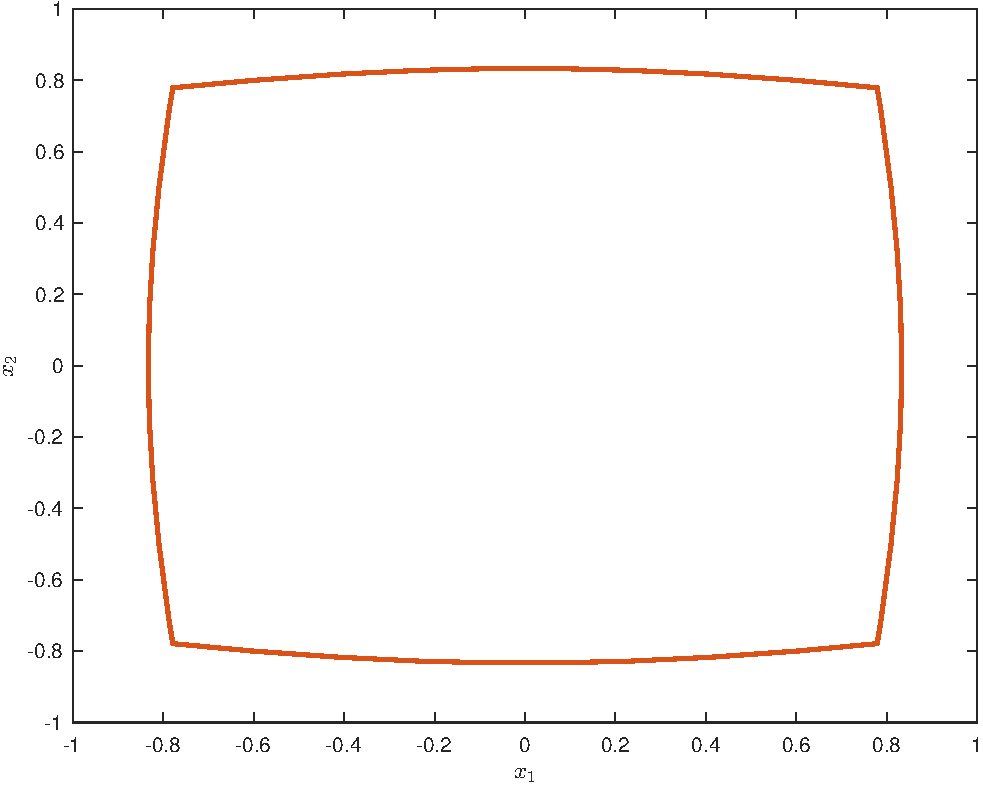
\includegraphics[width=.95\columnwidth]{parametricPD.pdf}
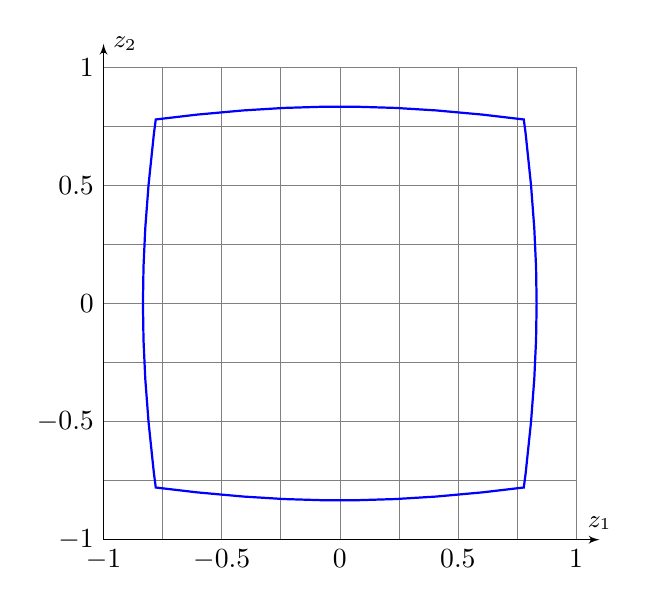
\begin{tikzpicture}[scale=3]
\draw[step=.25,gray,very thin] ( -1,  -1) grid (  1,   1);
\foreach \x in {-1,-0.5,...,1} \draw (\x,-1) node[below] {$\x$};
\foreach \y in {-1,-0.5,...,1} \draw (-1,\y) node[left] {$\y$};
\draw[thick,blue] (  0.0772,   0.8327) -- ( -0.0772,   0.8327) -- ( -0.2355,   0.8279) -- ( -0.4070,   0.8174) -- ( -0.6038,   0.7996) -- ( -0.7790,   0.7790) -- ( -0.7870,   0.7175) -- ( -0.8096,   0.5013) -- ( -0.8234,   0.3190) -- ( -0.8309,   0.1553) -- ( -0.8333,   0.0000) -- ( -0.8309,  -0.1553) -- ( -0.8234,  -0.3190) -- ( -0.8096,  -0.5013) -- ( -0.7870,  -0.7175) -- ( -0.7790,  -0.7790) -- ( -0.6038,  -0.7996) -- ( -0.4070,  -0.8174) -- ( -0.2355,  -0.8279) -- ( -0.0772,  -0.8327) -- (  0.0772,  -0.8327) -- (  0.2355,  -0.8279) -- (  0.4070,  -0.8174) -- (  0.6038,  -0.7996) -- (  0.7790,  -0.7790) -- (  0.7870,  -0.7175) -- (  0.8096,  -0.5013) -- (  0.8234,  -0.3190) -- (  0.8309,  -0.1553) -- (  0.8333,   0.0000) -- (  0.8309,   0.1553) -- (  0.8234,   0.3190) -- (  0.8096,   0.5013) -- (  0.7870,   0.7175) -- (  0.7790,   0.7790) -- (  0.6038,   0.7996) -- (  0.4070,   0.8174) -- (  0.2355,   0.8279) -- (  0.0772,   0.8327) -- cycle;
\draw[-latex'] (-1,-1) -- (1.1,-1) node[above] {\small{$z_1$}};
\draw[-latex'] (-1,-1) -- (-1,1.1) node[right] {\small{$z_2$}};
\end{tikzpicture}
\caption{$X\ominus\mathcal W(X)$ for Example~\ref{ssec:example:one}.}
\label{fig:example:parametric:pontryagin:difference}
\end{figure}


\subsection{Elementwise bound sets}\label{exp:second:example}
%
For another example we take inspiration from a robust control scenario.
%
We want to approximate the maximal positive invariant set for a system of the type~$x^+=Ax + f(x)$ for $x\in\mathcal X$, i.e. the largest set of points~$\mathcal X^\infty\subseteq\mathcal X$ such that $x\in\mathcal X^\infty\Rightarrow x^+\in\mathcal X^\infty$, see e.g.~\cite{blanchini:2007}.
%
For general nonlinear systems~$x^+=Ax + f(x)$ the maximal positive invariant set cannot be calculated, but assume we find piecewise affine bounds on the nonlinearity, i.e. $\min_{k\leq M_i}\{h_{i,k}^x x + h_{i,k}^c\}\leq f_i(x)\leq\max_{k\leq N_i}\{H_{i,k}^x x + H_{i,k}^c\}$ for all $x\in\mathcal X$ and all elements of~$f(x)$.
%
We can now study the system $x^+=Ax+w$ with $w\in\mathcal W(x) = \{w:\min_{k\leq M_i}\{h_{i,k}^x x + h_{i,k}^c\}\leq w_i\leq\max_{k\leq N_i}\{H_{i,k}^x x + H_{i,k}^c\}\,\forall i\in\mathbb N_d\}$.
%
To bound the maximal positive invariant set for the nonlinear system we compute the maximal robust positive invariant set for the perturbed linear system $x^+=Ax+w$, i.e. the set of states~$\mathscr X^\infty\subseteq\mathcal X$ such that $x\in\mathscr X^\infty$ implies $x^+\in\mathscr X^\infty$ for all possible $w\in\mathcal W(x)$.
%
The algorithm to determine the maximal robust positive invariant sets recursively intersects the current set iterate~$X_l$ with the set of all possible successor states starting from the current iterate $X_{l+1}=X_l\cap\left\{\bigcup_{x\in X_l,w\in\mathcal W(x)}\{Ax+w\}\right\}$.
%
We will only present a single step of this procedure.
%
Notice that for a constant set-valued map~$\mathcal W(x) = \mathcal W$ the iteration can be summarised as $X_{l+1} = X_l\cap A^{-1}(X_l\ominus\mathcal W)$, for a set valued map a similar compact notation also holds, however it is more confusing than helpful:~$X_{l+1}=X_l\cap(A^{-1}X_l\ominus A^{-1}\mathcal W(A^{-1}X_l))$.

In order to illustrate the proposed treatment of the nonlinearities we use the two dimensional system~$x^+=x+f(x)$ where the nonlinearity is given by
%
\begin{subequations}
\begin{equation}
  f_1(x) = \frac{1}{10}\left(\frac{x_1}{2}+x_2\right)^3
\end{equation}
\begin{equation}
  f_2(x) = \frac{1}{2}\arcsin\left(g_1\left(x_1-\frac{x_2}{2}\right)+g_2\left(x_1-\frac{x_2}{2}\right) \right)
\end{equation}
\end{subequations}
%
with $g_1(t)=\sigma(t)\sqrt{\frac{t}{2}}$, $g_2(t)=\sigma(-t)\frac{t}{2}$ where $\sigma(t)$ denotes the Heaviside function
%\sigma\left(x_1-\frac{x_2}{2}\right)\sqrt{\frac{x_1-\frac{x_2}{2}}{2}} + \sigma\left(-\left(x_1-\frac{x_2}{2}\right)\right)\frac{x_1-\frac{x_2}{2}}{2}
$$
  \sigma(t) = \left\{\begin{array}{crcl}1& t&\geq&0\\ 0 &t&<&0 \end{array}\right.
$$
%
As the constraint set we use $X_l = \{x:\abs{x_1}+\abs{x_2}\leq 2\}$.
%
We use piecewise affine approximations of $f_1(x)$~(Figure~\ref{fig:approximation:f1:p:diff}) and~$f_2(x)$ (Figure~\ref{fig:approximation:f2:p:diff})
% In order not to bore the reader with numerical values, we illustrate the approximation of $f_1(x)$ in Figure~\ref{fig:approximation:f1:p:diff} and~$f_2(x)$ in Figure~\ref{fig:approximation:f2:p:diff}, 
for both we obtain upper and lower bounds using secants and tangents.
%
Figure~\ref{fig:approximation:f2:p:diff} shows an obvious weakness of the approach:~$\max_k\{c_k x+b_k\}$ is necessarily convex, therefore approximating non-convex functions introduces conservativeness.

The computation of the set~$X_{l+1}$ is then done analogously to the previous example, again we use 
%
$$
  \mathcal W(x) = \conv\left\{\begin{pmatrix}t_1\\ t_3\end{pmatrix},\begin{pmatrix}t_1\\ t_4\end{pmatrix},
  \begin{pmatrix} t_2\\ t_3\end{pmatrix},\begin{pmatrix}t_2\\ t_4\end{pmatrix}
  \right\}
$$
%
with $t_1=\max_k\{H_{1,k}^x x+H_{1,k}^c\},\; t_3=\max_k\{H_{2,k}^x x+H_{2,k}^c\},\; t_2=-\max_k\{-h_{1,k}^x x-h_{1,k}^c\}$ and $t_4=-\max_k\{-h_{1,k}^x x-h_{1,k}^c\}$.
%
Each facet~$P_i=\{x:\Lambda_i x=\lambda_i\wedge\Lambda_jx\leq\lambda_j,j\neq i\}$ of the current set iterate defines facets of the next set iterate satisfying
%
\begin{equation}
\Lambda_i(Ax+w^\ast)=\lambda_i\quad \Lambda_j(Ax+w^\ast)\leq\lambda_j,j\neq i
\end{equation}
%
where $w^\ast$ is the maximiser of the defining mpLP $\max_{w\in\mathcal W(x)}\Lambda_iw$, i.e. one of the aforementioned vertices with their representation
%
$$
  \begin{pmatrix} w_1\\ \vdots \\ w_N\end{pmatrix}= Tt.
$$
%
With this the collection of facets generated by~$P_i$ is given by the projection
%
\begin{equation}
  \pi_d\left(\left\{(x,t,\tau):\begin{array}{rcl}
  \Lambda_iAx+\tau&=&\lambda_i\\
  \Lambda_i T_lt&\leq&\tau\\
  \Lambda_j(Ax+T_lt)&\leq&\lambda_j\\
  H_l^x x + H_l^c&\leq&t_{2l-1}\\
  -h_l^x x - h_l^c&\leq&t_{2l}
  \end{array}, \begin{array}{l}
  j\neq i\\
  l\in\mathbb N_d\end{array}
  \right\}\right)
\end{equation}
%
Analogously to the previous example, instead of computing~$q$ projections from $3d+1$ onto $d$ we can perform a single projection with the same result:
%
\begin{equation}
  \pi_d\left(\left\{(x,t,\tau):\begin{array}{rcl}
  \Lambda_i T_lt&\leq&\tau_i\\
  \Lambda_iAx+\tau_i&\leq&\lambda_i\\
  H_l^x x + H_l^c&\leq&t_{2l-1}\\
  -h_l^x x - h_l^c&\leq&t_{2l}
  \end{array}, \begin{array}{l}
  i\in\mathbb N_q,\\
  l\in\mathbb N_d\end{array}
  \right\}\right)
\end{equation}
%
The resulting set for this 2 dimensional example is illustrated in Figure~\ref{fig:second:example:resulting:set}.


\begin{figure}
\centering
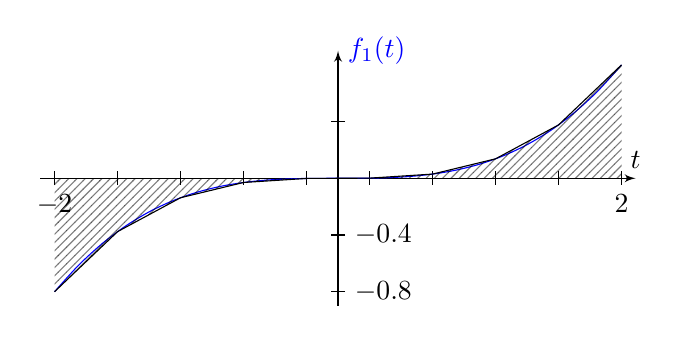
\begin{tikzpicture}[scale=1.8]
\draw[-latex'] (-2.1,0) -- (2.1,0) node[above] {$t$};
\draw[-latex'] (0,-.9) -- (0,.9) node[right,blue] {$f_1(t)$};
\foreach \x in {-2,-1.5556,...,2} \draw (\x,0.05) -- (\x,-.05);
\draw (-2,-.05) node[below] {$-2$};
\draw (2,-.05) node[below] {$2$};
\foreach \y in {-.8,-.4,...,.8} \draw (0.05,\y) -- (-.05,\y);
\draw (.05,-.8) node[right] {$-0.8$};
\draw (.05,-.4) node[right] {$-0.4$};
\draw[scale=1,domain=-2:2,smooth,variable=\x,blue] plot ({\x},{\x*\x*\x/10});
\draw (-2.0000, -0.8000) -- (-1.5556, -0.3764) -- (-1.1111, -0.1372) -- (-0.6667, -0.0296) -- (-0.2222, -0.0011) -- (0,0); 
\draw (0,0) -- (0.2222, 0.0011) -- (0.6667, 0.0296) -- (1.1111, 0.1372) -- (1.5556, 0.3764) -- (2.0000, 0.8000);
\fill[pattern = north east lines, opacity=.5] (-2.0000, -0.8000) -- (-1.5556, -0.3764) -- (-1.1111, -0.1372) -- (-0.6667, -0.0296) -- (-0.2222, -0.0011) -- (0,0) -- (-2,0) -- cycle; 
\fill[pattern = north east lines, opacity=.5] (0,0) -- (0.2222, 0.0011) -- (0.6667, 0.0296) -- (1.1111, 0.1372) -- (1.5556, 0.3764) -- (2.0000, 0.8000) -- (2,0) -- cycle;
\end{tikzpicture}
\caption{$f_1(t)$, for $t=\frac{x_1}{2}+x_2$, and its approximation by 9 secants used in Example~\ref{exp:second:example}.}
\label{fig:approximation:f1:p:diff}
\end{figure}

\begin{figure}
\centering
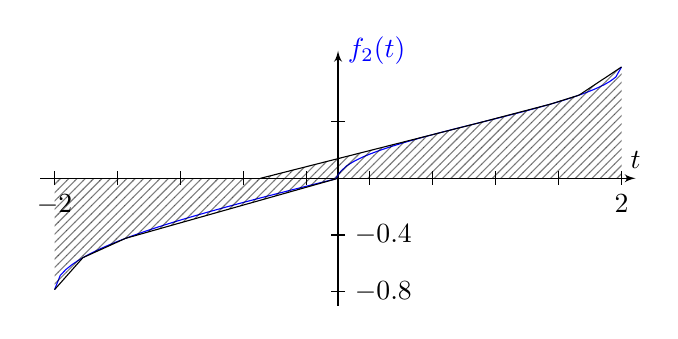
\begin{tikzpicture}[scale=1.8]
\draw[-latex'] (-2.1,0) -- (2.1,0) node[above] {$t$};
\draw[-latex'] (0,-.9) -- (0,.9) node[right,blue] {$f_2(t)$};
\foreach \x in {-2,-1.5556,...,2} \draw (\x,0.05) -- (\x,-.05);
\draw (-2,-.05) node[below] {$-2$};
\draw (2,-.05) node[below] {$2$};
\foreach \y in {-.8,-.4,...,.8} \draw (0.05,\y) -- (-.05,\y);
\draw (.05,-.8) node[right] {$-0.8$};
\draw (.05,-.4) node[right] {$-0.4$};
\draw[blue] (-2.0000, -0.7854) -- (-1.9596, -0.6847) -- (-1.9192, -0.6428) -- (-1.8788, -0.6104) -- (-1.8384, -0.5830) -- (-1.7980, -0.5587) -- (-1.7576, -0.5367) -- (-1.7172, -0.5163) -- (-1.6768, -0.4972) -- (-1.6364, -0.4791) -- (-1.5960, -0.4620) -- (-1.5556, -0.4456) -- (-1.5152, -0.4298) -- (-1.4747, -0.4146) -- (-1.4343, -0.3999) -- (-1.3939, -0.3856) -- (-1.3535, -0.3717) -- (-1.3131, -0.3581) -- (-1.2727, -0.3449) -- (-1.2323, -0.3319) -- (-1.1919, -0.3192) -- (-1.1515, -0.3068) -- (-1.1111, -0.2945) -- (-1.0707, -0.2825) -- (-1.0303, -0.2706) -- (-0.9899, -0.2589) -- (-0.9495, -0.2473) -- (-0.9091, -0.2359) -- (-0.8687, -0.2247) -- (-0.8283, -0.2135) -- (-0.7879, -0.2025) -- (-0.7475, -0.1915) -- (-0.7071, -0.1807) -- (-0.6667, -0.1699) -- (-0.6263, -0.1592) -- (-0.5859, -0.1486) -- (-0.5455, -0.1381) -- (-0.5051, -0.1276) -- (-0.4646, -0.1172) -- (-0.4242, -0.1069) -- (-0.3838, -0.0966) -- (-0.3434, -0.0863) -- (-0.3030, -0.0761) -- (-0.2626, -0.0658) -- (-0.2222, -0.0557) -- (-0.1818, -0.0455) -- (-0.1414, -0.0354) -- (-0.1010, -0.0253) -- (-0.0606, -0.0152) -- (-0.0202, -0.0051) -- ( 0.0202,  0.0503) -- ( 0.0606,  0.0875) -- ( 0.1010,  0.1133) -- ( 0.1414,  0.1346) -- ( 0.1818,  0.1531) -- ( 0.2222,  0.1699) -- ( 0.2626,  0.1854) -- ( 0.3030,  0.1999) -- ( 0.3434,  0.2136) -- ( 0.3838,  0.2267) -- ( 0.4242,  0.2393) -- ( 0.4646,  0.2515) -- ( 0.5051,  0.2633) -- ( 0.5455,  0.2747) -- ( 0.5859,  0.2859) -- ( 0.6263,  0.2969) -- ( 0.6667,  0.3077) -- ( 0.7071,  0.3184) -- ( 0.7475,  0.3289) -- ( 0.7879,  0.3393) -- ( 0.8283,  0.3496) -- ( 0.8687,  0.3598) -- ( 0.9091,  0.3699) -- ( 0.9495,  0.3801) -- ( 0.9899,  0.3902) -- ( 1.0303,  0.4003) -- ( 1.0707,  0.4104) -- ( 1.1111,  0.4205) -- ( 1.1515,  0.4307) -- ( 1.1919,  0.4410) -- ( 1.2323,  0.4513) -- ( 1.2727,  0.4618) -- ( 1.3131,  0.4723) -- ( 1.3535,  0.4830) -- ( 1.3939,  0.4939) -- ( 1.4343,  0.5050) -- ( 1.4747,  0.5164) -- ( 1.5152,  0.5280) -- ( 1.5556,  0.5400) -- ( 1.5960,  0.5523) -- ( 1.6364,  0.5651) -- ( 1.6768,  0.5785) -- ( 1.7172,  0.5926) -- ( 1.7576,  0.6076) -- ( 1.7980,  0.6237) -- ( 1.8384,  0.6413) -- ( 1.8788,  0.6610) -- ( 1.9192,  0.6842) -- ( 1.9596,  0.7141) -- ( 2.0000,  0.7854);
\draw (-2.0000, -0.7854) -- (-1.8000, -0.5599) -- (-1.5000, -0.4240) -- (0, 0);
\fill[pattern = north east lines, opacity=.5] (-2.0000, -0.7854) -- (-1.8000, -0.5599) -- (-1.5000, -0.4240) -- (0, 0) -- (-2,0) -- cycle;
\draw (-.5466,0) -- (0.7000, 0.3165) -- (1.0000, 0.3927) -- (1.5000, 0.5236) -- (1.7000, 0.5865) -- (2.0000, 0.7854);
\fill[pattern = north east lines, opacity=.5] (-.5466,0) -- (0.7000, 0.3165) -- (1.0000, 0.3927) -- (1.5000, 0.5236) -- (1.7000, 0.5865) -- (2.0000, 0.7854) -- (2,0) -- cycle;
\end{tikzpicture}
\caption{$f_2(t)$, for $t=x_1-\frac{x_2}{2}$, and its approximation by 5 secants and 4 tangents as used in Example~\ref{exp:second:example}.}
\label{fig:approximation:f2:p:diff}
\end{figure}

\begin{figure}
\centering
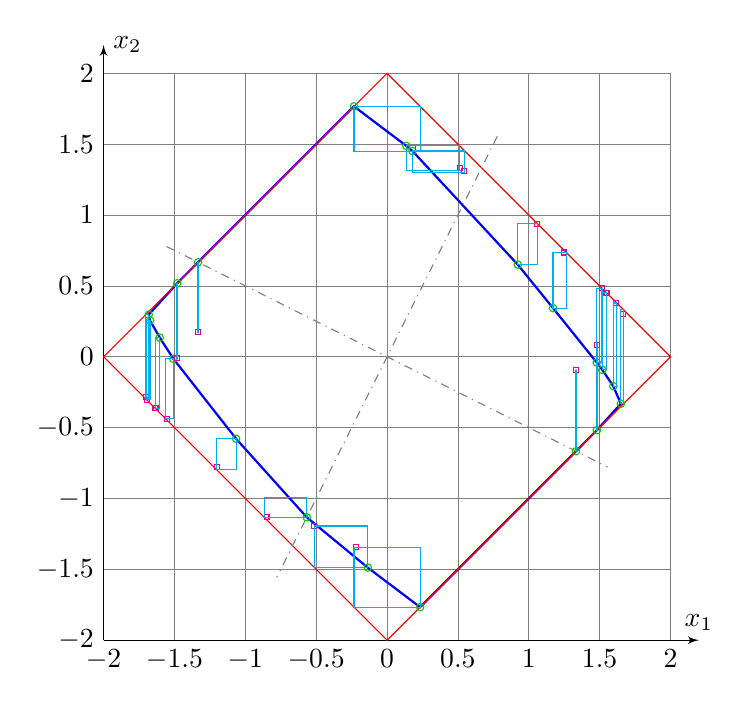
\begin{tikzpicture}[scale=1.8]
\draw[step=.5,gray,very thin] (-2,-2) grid (2,2);
\foreach \x in {-2,-1.5,...,2} \draw (\x,-2) node[below] {$\x$};
\foreach \y in {-2,-1.5,...,2} \draw (-2,\y) node[left] {$\y$};
\draw[-latex'] (-2,-2) -- (2.2,-2) node[above] {$x_1$};
\draw[-latex'] (-2,-2) -- (-2,2.2) node[right] {$x_2$};
\draw[blue,thick] ( -0.2333,   1.7667) -- ( -1.3333,   0.6667) -- ( -1.4807,   0.5182) -- ( -1.6815,   0.2968) -- ( -1.6720,   0.2560) -- ( -1.6039,   0.1353) -- ( -1.5073,  -0.0145) -- ( -1.0649,  -0.5786) -- ( -0.5663,  -1.1326) -- ( -0.1361,  -1.4875) -- (  0.2333,  -1.7667) -- (  1.3333,  -0.6667) -- (  1.4807,  -0.5182) -- (  1.6499,  -0.3316) -- (  1.5962,  -0.2075) -- (  1.5190,  -0.0928) -- (  1.4796,  -0.0407) -- (  1.1714,   0.3429) -- (  0.9224,   0.6499) -- (  0.1793,   1.4518) -- (  0.1361,   1.4875) -- ( -0.2333,   1.7667) -- cycle;
\draw[red] (  2.0000,   0.0000) -- (  0.0000,   2.0000) -- ( -2.0000,  -0.0000) -- ( -0.0000,  -2.0000) -- (  2.0000,   0.0000) -- cycle;
\foreach \x/\y in { -0.2333/  1.7667,  0.1361/  1.4875,  0.1793/  1.4518, -1.3333/  0.6667, -1.0649/ -0.5786, -1.5073/ -0.0145, -1.6039/  0.1353,  0.9224/  0.6499,  1.6499/ -0.3316,  1.4807/ -0.5182,  1.5962/ -0.2075,  1.4796/ -0.0407,  1.5190/ -0.0928,  1.3333/ -0.6667,  1.1714/  0.3429,  0.2333/ -1.7667, -0.1361/ -1.4875, -0.5663/ -1.1326, -1.6720/  0.2560, -1.6815/  0.2968, -1.4807/  0.5182} \draw[green!80!black] (\x,\y) circle (.75pt);
\foreach \x/\y in {  0.2160/  1.4706,  0.5125/  1.3332,  0.5456/  1.3134, -1.3333/  0.1741, -1.2021/ -0.7778, -1.5526/ -0.4386, -1.6336/ -0.3595,  1.0596/  0.9390,  1.6619/  0.2996,  1.4818/  0.0827,  1.6168/  0.3790,  1.5138/  0.4829,  1.5486/  0.4501,  1.3333/ -0.0915,  1.2515/  0.7356, -0.2160/ -1.3448, -0.5125/ -1.1956, -0.8500/ -1.1326, -1.6915/ -0.3039, -1.6976/ -0.2809, -1.4818/ -0.0094} \draw[yshift=-.5pt,xshift=-.5pt,magenta] (\x,\y) rectangle ++(1pt,1pt);
% \foreach \x/\y in {0.2333/  1.7667,  0.2333/  1.4511, -0.2333/  1.7667, -0.2333/  1.4511,  0.5125/  1.4875,  0.5125/  1.3157,  0.1361/  1.4875,  0.1361/  1.3157,  0.5482/  1.4518,  0.5482/  1.2973,  0.1793/  1.4518,  0.1793/  1.2973, -1.3333/  0.6667, -1.3333/  0.1672, -1.3333/  0.6667, -1.3333/  0.1672, -1.0649/ -0.5786, -1.0649/ -0.7979, -1.2021/ -0.5786, -1.2021/ -0.7979, -1.5073/ -0.0145, -1.5073/ -0.4386, -1.5614/ -0.0145, -1.5614/ -0.4386, -1.6039/  0.1353, -1.6039/ -0.3664, -1.6336/  0.1353, -1.6336/ -0.3664,  1.0596/  0.9404,  1.0596/  0.6499,  0.9224/  0.9404,  0.9224/  0.6499,  1.6684/  0.3316,  1.6684/ -0.3316,  1.6499/  0.3316,  1.6499/ -0.3316,  1.4818/  0.0948,  1.4818/ -0.5182,  1.4807/  0.0948,  1.4807/ -0.5182,  1.6210/  0.3790,  1.6210/ -0.2075,  1.5962/  0.3790,  1.5962/ -0.2075,  1.5171/  0.4829,  1.5171/ -0.0407,  1.4796/  0.4829,  1.4796/ -0.0407,  1.5486/  0.4514,  1.5486/ -0.0928,  1.5190/  0.4514,  1.5190/ -0.0928,  1.3333/ -0.0906,  1.3333/ -0.6667,  1.3333/ -0.0906,  1.3333/ -0.6667,  1.2644/  0.7356,  1.2644/  0.3429,  1.1714/  0.7356,  1.1714/  0.3429,  0.2333/ -1.3435,  0.2333/ -1.7667, -0.2333/ -1.3435, -0.2333/ -1.7667, -0.1361/ -1.1944, -0.1361/ -1.4875, -0.5125/ -1.1944, -0.5125/ -1.4875, -0.5663/ -0.9938, -0.5663/ -1.1326, -0.8674/ -0.9938, -0.8674/ -1.1326, -1.6720/  0.2560, -1.6720/ -0.3039, -1.6961/  0.2560, -1.6961/ -0.3039, -1.6815/  0.2968, -1.6815/ -0.2968, -1.7032/  0.2968, -1.7032/ -0.2968, -1.4807/  0.5182, -1.4807/ -0.0145, -1.4818/  0.5182, -1.4818/ -0.0145} {
%   \draw[cyan] (\x-.02,\y-.02) -- (\x+.02,\y+.02); 
%   \draw[cyan] (\x-.02,\y+.02) -- (\x+.02,\y-.02);
%   }

\draw[cyan] (  0.2333,  1.7667) -- (  0.2333,  1.4511) -- ( -0.2333,  1.4511) -- ( -0.2333,  1.7667) -- cycle;
\draw[cyan] (  0.5125,  1.4875) -- (  0.5125,  1.3157) -- (  0.1361,  1.3157) -- (  0.1361,  1.4875) -- cycle;
\draw[cyan] (  0.5482,  1.4518) -- (  0.5482,  1.2973) -- (  0.1793,  1.2973) -- (  0.1793,  1.4518) -- cycle;
\draw[cyan] ( -1.3333,  0.6667) -- ( -1.3333,  0.1672) -- ( -1.3333,  0.1672) -- ( -1.3333,  0.6667) -- cycle;
\draw[cyan] ( -1.0649, -0.5786) -- ( -1.0649, -0.7979) -- ( -1.2021, -0.7979) -- ( -1.2021, -0.5786) -- cycle;
\draw[cyan] ( -1.5073, -0.0145) -- ( -1.5073, -0.4386) -- ( -1.5614, -0.4386) -- ( -1.5614, -0.0145) -- cycle;
\draw[cyan] ( -1.6039,  0.1353) -- ( -1.6039, -0.3664) -- ( -1.6336, -0.3664) -- ( -1.6336,  0.1353) -- cycle;
\draw[cyan] (  1.0596,  0.9404) -- (  1.0596,  0.6499) -- (  0.9224,  0.6499) -- (  0.9224,  0.9404) -- cycle;
\draw[cyan] (  1.6684,  0.3316) -- (  1.6684, -0.3316) -- (  1.6499, -0.3316) -- (  1.6499,  0.3316) -- cycle;
\draw[cyan] (  1.4818,  0.0948) -- (  1.4818, -0.5182) -- (  1.4807, -0.5182) -- (  1.4807,  0.0948) -- cycle;
\draw[cyan] (  1.6210,  0.3790) -- (  1.6210, -0.2075) -- (  1.5962, -0.2075) -- (  1.5962,  0.3790) -- cycle;
\draw[cyan] (  1.5171,  0.4829) -- (  1.5171, -0.0407) -- (  1.4796, -0.0407) -- (  1.4796,  0.4829) -- cycle;
\draw[cyan] (  1.5486,  0.4514) -- (  1.5486, -0.0928) -- (  1.5190, -0.0928) -- (  1.5190,  0.4514) -- cycle;
\draw[cyan] (  1.3333, -0.0906) -- (  1.3333, -0.6667) -- (  1.3333, -0.6667) -- (  1.3333, -0.0906) -- cycle;
\draw[cyan] (  1.2644,  0.7356) -- (  1.2644,  0.3429) -- (  1.1714,  0.3429) -- (  1.1714,  0.7356) -- cycle;
\draw[cyan] (  0.2333, -1.3435) -- (  0.2333, -1.7667) -- ( -0.2333, -1.7667) -- ( -0.2333, -1.3435) -- cycle;
\draw[cyan] ( -0.1361, -1.1944) -- ( -0.1361, -1.4875) -- ( -0.5125, -1.4875) -- ( -0.5125, -1.1944) -- cycle;
\draw[cyan] ( -0.5663, -0.9938) -- ( -0.5663, -1.1326) -- ( -0.8674, -1.1326) -- ( -0.8674, -0.9938) -- cycle;
\draw[cyan] ( -1.6720,  0.2560) -- ( -1.6720, -0.3039) -- ( -1.6961, -0.3039) -- ( -1.6961,  0.2560) -- cycle;
\draw[cyan] ( -1.6815,  0.2968) -- ( -1.6815, -0.2968) -- ( -1.7032, -0.2968) -- ( -1.7032,  0.2968) -- cycle;
\draw[cyan] ( -1.4807,  0.5182) -- ( -1.4807, -0.0145) -- ( -1.4818, -0.0145) -- ( -1.4818,  0.5182) -- cycle;


\draw[thin,dash dot,gray] (0.7778,1.5556) -- (-0.7778,-1.5556);
\draw[thin,dash dot,gray] (-1.5556,0.7778) -- (1.5556,-0.7778);
\end{tikzpicture}
% \caption[The parametric Pontryagin difference of a parametrically convex PWA set-valued map.]{The resulting set~$\mathcal X\ominus\mathcal W(\mathcal X)$ for Example~\ref{example:most:complex:pontryagin:difference:ever} in \textcolor{blue}{blue}, its vertices~$v_i$ marked by \textcolor{green!80!black}{green} circles, in \textcolor{red}{red} the set~$\mathcal X$, \textcolor{cyan}{cyan} boxes outline $\{v_i\}\oplus\mathcal W(v_i)$, \textcolor{magenta}{magenta} rectangles mark the actual value of $f(v_i)$, notice that each~$f(v_i)\in\{v_i\}\oplus\mathcal W(v_i)$ as required, and dash-dotted lines show the $x_1-\frac{x_2}{2}=0$ and $\frac{x_1}{2}+x_2=0$ planes.}


% 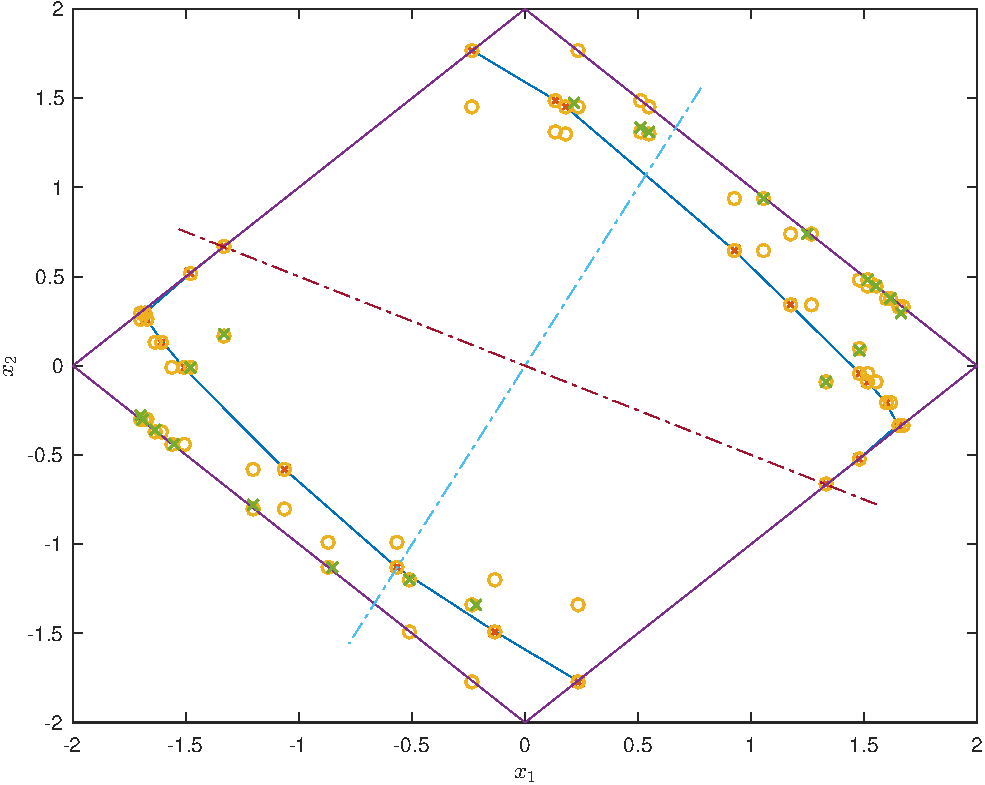
\includegraphics[width=.95\textwidth]{complexPonDiff.pdf}
\caption{In red~$X_l$, outlined in blue~$X_{l+1}$, its vertices~$v_i$ marked by green circles, in cyan we outline $\{v_i\}\oplus\mathcal W(v_i)$, the red squares mark the actual value of $f(v_i)$ and dotted lines show the $x_1-\frac{x_2}{2}=0$ and $\frac{x_1}{2}+x_2=0$ planes.}
\label{fig:second:example:resulting:set}
\end{figure}
%
%
%
%
%
\section{Conclusion}\label{sec:conclusion}
%
%
%
In this paper we present a way to extend the scope of the Pontryagin
difference operation to a wide class of sets and set-valued maps.
%
We introduce the framework of parametric convexity and related analysis, which proves essential for the convexity of the parametric Pontryagin difference.
%
Furthermore we provide the link required to make the parametric Pontryagin difference computationally accessible for polytopic sets, this relies on the combinatorial nature of the subtrahend set-valued map.
%
Using two simple examples we illustrated the potency of the proposed methodology.

The parametric Pontryagin difference has been applied successfully in a robust control environment~\cite{Schaich:2015,Schaich:2015a} and this work will further to extend its scope of application.

\bibliographystyle{plain}
\bibliography{Bibliography}

\end{document}